\documentclass[oneside,b5papar,11pt]{book}

\usepackage[protrusion=true,expansion=true]{microtype} % Better typography
\usepackage{graphicx,wrapfig} % Required for including pictures
\usepackage{mathpazo} % Use the Palatino font
\usepackage[T1]{fontenc} % Required for accented characters
\usepackage{amscd,amsmath}
\usepackage{tikz,stmaryrd}
\usepackage{latexsym,amsbsy,bbold, fullpage}
\usepackage{amssymb,amsthm,amsfonts}
\usepackage{pdfsync,yfonts}
\usepackage{tkz-graph,tikz-cd}
\usepackage[all,pdf]{xy}
\usepackage{ctex}
\usepackage{titlesec}
\usepackage{color,xcolor,tcolorbox}
\usepackage{framed}
\usepackage{hyperref,url}
\usepackage{makeidx}
\usepackage[annataritalic]{tengwarscript}%支持Tengwa字母,可以写精灵语了
\usepackage{enumitem}

\def\UrlBreaks{\do\A\do\B\do\C\do\D\do\E\do\F\do\G\do\H\do\I\do\J
\do\K\do\L\do\M\do\N\do\O\do\P\do\Q\do\R\do\S\do\T\do\U\do\V
\do\W\do\X\do\Y\do\Z\do\[\do\\\do\]\do\^\do\_\do\`\do\a\do\b
\do\c\do\d\do\e\do\f\do\g\do\h\do\i\do\j\do\k\do\l\do\m\do\n
\do\o\do\p\do\q\do\r\do\s\do\t\do\u\do\v\do\w\do\x\do\y\do\z
\do\.\do\@\do\\\do\/\do\!\do\_\do\|\do\;\do\>\do\]\do\)\do\,
\do\?\do\'\do+\do\=\do\#}%URL换行咒语

\usetikzlibrary{matrix, calc, arrows}
\usetikzlibrary{patterns,trees,snakes}

\makeindex

%%%%%%%%%%%%%%%%%%%%%%%%%%%%%%%%%%%%%%%%%%%%%%%%%%%%
%在此处调整 定义、定理、性质、引理、公理 的背景颜色%
\newcommand{\chapterbackgroundcolor}{
  \definecolor{shadecolor}{RGB}{255,227,170}
}

\newcommand*{\thmcolor}{185,181,134}
\newcommand*{\propcolor}{201,198,160}
\newcommand*{\lemmacolor}{225,225,200}
\newcommand*{\axiomcolor}{247,247,249}
\newcommand*{\definitioncolor}{173,197,165}
\newcommand*{\notationcolor}{208,222,203}
%%%%%%%%%%%%%%%%%%%%%%%%%%%%%%%%%%%%%%%%%%%%%%%%%%%%

%%%%%%%%%%%%%%%%%%%%%%%%%%%%%%%%%%%%
%%%%%这里调用了曲豆豆的独家秘籍%%%%%
%这是曲豆豆的红包

%%%%%%%%%%%%%%定理环境%%%%%%%%%%%%%%%%%%%%%%%

\newtheorem{mythm}{定理}[section]
\newtheorem{mylemma}[mythm]{引理}
\newtheorem{myprop}[mythm]{性质}
\newtheorem{myaxiom}[mythm]{公理}
\newtheorem{mydefinition}[mythm]{定义}
\newtheorem{mynotation}[mythm]{记号}
\newtheorem{example}[mythm]{例子}
\newtheorem{PreImportantExample}[mythm]{重要例子}
\newtheorem{rem}[mythm]{注记}
\newtheorem{mycor}[mythm]{推论}
\newtheorem{claim}[mythm]{断言}
\newtheorem{prob}{习题}[section]


\chapterbackgroundcolor


\newenvironment{thm}
  {\definecolor{shadecolor}{RGB}{\thmcolor}
    \begin{shaded}\begin{mythm}}
  {\end{mythm}\end{shaded}
  \chapterbackgroundcolor}

\newenvironment{lemma}
  {\definecolor{shadecolor}{RGB}{\lemmacolor}
    \begin{shaded}\begin{mylemma}}
  {\end{mylemma}\end{shaded}
  \chapterbackgroundcolor}

\newenvironment{prop}
  {\definecolor{shadecolor}{RGB}{\propcolor}
    \begin{shaded}\begin{myprop}}
  {\end{myprop}\end{shaded}
  \chapterbackgroundcolor}

\newenvironment{axiom}
  {\definecolor{shadecolor}{RGB}{\axiomcolor}
    \begin{shaded}\begin{myaxiom}}
  {\end{myaxiom}\end{shaded}
  \chapterbackgroundcolor}

\newenvironment{cor}
  {\definecolor{shadecolor}{RGB}{\lemmacolor}
    \begin{shaded}\begin{mycor}}
  {\end{mycor}\end{shaded}
  \chapterbackgroundcolor}

\newenvironment{definition}
  {\definecolor{shadecolor}{RGB}{\definitioncolor}
    \begin{shaded}\begin{mydefinition}}
  {\end{mydefinition}\end{shaded}
  \chapterbackgroundcolor}

\newenvironment{notation}
  {\definecolor{shadecolor}{RGB}{\notationcolor}
    \begin{shaded}\begin{mynotation}}
  {\end{mynotation}\end{shaded}
  \chapterbackgroundcolor}

\newenvironment{Example}
  {\definecolor{shadecolor}{RGB}{\examplecolor}
    \begin{shaded}\begin{PreImportantExample}}
  {\end{PreImportantExample}\end{shaded}
  \chapterbackgroundcolor}

%%%%%%%%%%%%%%%%%%%%%%%%%%%%%%%%%%%%%%%%%%%%%%%%%%%%%%%%%%%%
\newcommand*{\vs}{\vspace{5pt}}
\newcommand*{\vsp}{\vspace{10pt}}
\newcommand*{\vspp}{\vspace{20pt}}
\newcommand*{\kong}{$\,\,\,$}
\newcommand*{\fengexian}{
  \rule[0pt]{14.3cm}{0.01em}
\vs}
%%%%%%%%%%%%%%%%%%%%%%%%%%%%%%%%%%%%%%%%%%%%%%%%%%%%%%%%%%%%
\newcommand*{\Langle}{\left\langle}
\newcommand*{\Rangle}{\right\rangle}
%%%%%%%%%%%%%%%%%%%%%%%%%%%%%%%%%%%%%%%%%%%%%%%%%%%%%%%%%%%%
\newcommand*{\bbA}{\mathbb{A}}
\newcommand*{\bbB}{\mathbb{B}}
\newcommand*{\bbC}{\mathbb{C}}
\newcommand*{\bbD}{\mathbb{D}}
\newcommand*{\bbE}{\mathbb{E}}
\newcommand*{\bbF}{\mathbb{F}}
\newcommand*{\bbG}{\mathbb{G}}
\newcommand*{\bbH}{\mathbb{H}}
\newcommand*{\bbI}{\mathbb{I}}
\newcommand*{\bbJ}{\mathbb{J}}
\newcommand*{\bbK}{\mathbb{K}}
\newcommand*{\bbL}{\mathbb{L}}
\newcommand*{\bbM}{\mathbb{M}}
\newcommand*{\bbN}{\mathbb{N}}
\newcommand*{\bbO}{\mathbb{O}}
\newcommand*{\bbP}{\mathbb{P}}
\newcommand*{\bbQ}{\mathbb{Q}}
\newcommand*{\bbR}{\mathbb{R}}
\newcommand*{\bbS}{\mathbb{S}}
\newcommand*{\bbT}{\mathbb{T}}
\newcommand*{\bbU}{\mathbb{U}}
\newcommand*{\bbV}{\mathbb{V}}
\newcommand*{\bbW}{\mathbb{W}}
\newcommand*{\bbX}{\mathbb{X}}
\newcommand*{\bbY}{\mathbb{Y}}
\newcommand*{\bbZ}{\mathbb{Z}}

\newcommand*{\mcalA}{\mathcal{A}}
\newcommand*{\mcalB}{\mathcal{B}}
\newcommand*{\mcalC}{\mathcal{C}}
\newcommand*{\mcalD}{\mathcal{D}}
\newcommand*{\mcalE}{\mathcal{E}}
\newcommand*{\mcalF}{\mathcal{F}}
\newcommand*{\mcalG}{\mathcal{G}}
\newcommand*{\mcalH}{\mathcal{H}}
\newcommand*{\mcalI}{\mathcal{I}}
\newcommand*{\mcalJ}{\mathcal{J}}
\newcommand*{\mcalK}{\mathcal{K}}
\newcommand*{\mcalL}{\mathcal{L}}
\newcommand*{\mcalM}{\mathcal{M}}
\newcommand*{\mcalN}{\mathcal{N}}
\newcommand*{\mcalO}{\mathcal{O}}
\newcommand*{\mcalP}{\mathcal{P}}
\newcommand*{\mcalQ}{\mathcal{Q}}
\newcommand*{\mcalR}{\mathcal{R}}
\newcommand*{\mcalS}{\mathcal{S}}
\newcommand*{\mcalT}{\mathcal{T}}
\newcommand*{\mcalU}{\mathcal{U}}
\newcommand*{\mcalV}{\mathcal{V}}
\newcommand*{\mcalW}{\mathcal{W}}
\newcommand*{\mcalX}{\mathcal{X}}
\newcommand*{\mcalY}{\mathcal{Y}}
\newcommand*{\mcalZ}{\mathcal{Z}}

\newcommand*{\mfkg}{\mathfrak{g}}    %Lie algebra
\newcommand*{\mfkh}{\mathfrak{h}}
\newcommand*{\mfkm}{\mathfrak{m}}    %maximal ideal
\newcommand*{\mfkp}{\mathfrak{p}}    %prime ideal
\newcommand*{\mfkq}{\mathfrak{q}}

\newcommand*{\mfkgl}{\mathfrak{gl}}
\newcommand*{\mfksl}{\mathfrak{sl}}
\newcommand*{\mfkso}{\mathfrak{so}}
\newcommand*{\mfksp}{\mathfrak{sp}}

\newcommand*{\bfk}{\boldsymbol{k}}
\newcommand*{\bfp}{\boldsymbol{p}}
\newcommand*{\bfq}{\boldsymbol{q}}
\newcommand*{\bfu}{\boldsymbol{u}}
\newcommand*{\bfv}{\boldsymbol{v}}
\newcommand*{\bfw}{\boldsymbol{w}}
\newcommand*{\bfx}{\boldsymbol{x}}
\newcommand*{\bfy}{\boldsymbol{y}}
\newcommand*{\bfz}{\boldsymbol{z}}

\newcommand*{\Ahat}{\hat{A}}
\newcommand*{\Bhat}{\hat{B}}
\newcommand*{\Chat}{\hat{C}}
\newcommand*{\Dhat}{\hat{D}}
\newcommand*{\Ehat}{\hat{E}}
\newcommand*{\Fhat}{\hat{F}}
\newcommand*{\Ghat}{\hat{G}}
\newcommand*{\Hhat}{\hat{H}}

\newcommand*{\zbar}{\overline{z}}            %complex number
\newcommand*{\wbar}{\overline{w}}
\newcommand*{\taubar}{\overline{\tau}}

\newcommand*{\ftil}{\widetilde{f}}
\newcommand*{\gtil}{\widetilde{g}}
\newcommand*{\htil}{\widetilde{h}}
\newcommand*{\itil}{\widetilde{i}}
\newcommand*{\xtil}{\widetilde{x}}
\newcommand*{\ytil}{\widetilde{y}}
\newcommand*{\ztil}{\widetilde{z}}
\newcommand*{\wtil}{\widetilde{w}}

\newcommand*{\Omgtil}{\widetilde{\Omega}}

\newcommand*{\afa}{\alpha}
\newcommand*{\lmd}{\lambda}
\newcommand*{\Lmd}{\Lambda}
\newcommand*{\sgm}{\sigma}
\newcommand*{\Sgm}{\Sigma}
\newcommand*{\gma}{\gamma}
\newcommand*{\Gma}{\Gamma}
\newcommand*{\dta}{\delta}
\newcommand*{\Dta}{\Delta}
\newcommand*{\omg}{\omega}
\newcommand*{\Omg}{\Omega}
\newcommand*{\veps}{\varepsilon}
\newcommand*{\fai}{\varphi}
\newcommand*{\pai}{\varpi}

%%%%%%%%%%%%%%%%%%%%%%%%%%%%%%%%%%%%%%%%%%%%%%%%

\newcommand*{\ra}{\rightarrow}
\newcommand*{\inj}{\hookrightarrow}
\newcommand*{\surj}{\twoheadrightarrow}
\newcommand*{\xra}{\xrightarrow}
\newcommand*{\xla}{\xleftarrow}
\newcommand*{\llra}{\longleftrightarrow}
\newcommand*{\Llra}{\Longleftrightarrow}
\newcommand*{\rlim}{\varinjlim}                 %colimit,余极限,归纳极限,正向极限
\newcommand*{\llim}{\varprojlim}                %limit,极限,投射极限,逆向极限
\newcommand*{\suobing}{\lrcorner\,}             %张量的缩并

\newcommand*{\xybigrow}{\xymatrixrowsep{5pc}}   %交换图排版专用
\newcommand*{\xybigcol}{\xymatrixcolsep{5pc}}   %增大行、列间距
\newcommand*{\tabularbigrow}{\specialrule{0em}{4pt}{4pt}}

\newcommand*{\pz}{\text{---}}                   %破折号
\newcommand*{\yc}{\triangle}                    %余代数的乘法,co-product
\newcommand*{\p}{\partial}                      %偏微分、边缘算子partial
\newcommand*{\td}{\mathrm{d}}                   %微分算子d
\newcommand*{\pbar}{\overline{\partial}}        %Dolbeaut算子partial-bar
\newcommand*{\ten}{\otimes}                     %张量积tensor product
\newcommand*{\bigten}{\bigotimes}
\newcommand*{\op}{^{\text{op}}}
\newcommand*{\downdot}{_{\bullet}}              %下方黑点,用于同调代数中的链复形
\newcommand*{\ddowndot}{_{\bullet\bullet}}
\newcommand*{\updot}{^{\bullet}}
\newcommand*{\wedgeform}{\bigwedge\nolimits^}
\newcommand*{\ssubset}{\subset\!\subset}        %紧包含
\newcommand*{\vkong}{\varnothing}               %空集

%%%%%%%%%%%%%%%%%%%%%%%%%%%%%%%%%%%%%%%%%%%%%%%%
\newcommand*{\lbar}[1]{\overline{#1}}    %比较长的上横线

\newcommand*{\fps}[1]{[\![#1]\!]}        %Formal power series形式幂级数
\newcommand*{\Ls}[1]{(\!(#1)\!)}         %Laurent series     洛朗级数

\newcommand*{\Choose}[2]
  {\left[{
      #1 \atop
      #2
  }\right]}                              %快速输入小型方括号组合数

\newcommand*{\bbar}[1]
  {\overline{#1}}

\newcommand*{\pp}[1]
  {\frac{\partial   }
        {\partial #1}
  }                               %切向量场,一阶偏微分算子

\newcommand*{\pfrac}[2]
  {\frac{\partial #1}
        {\partial #2}
  }                               %一阶偏微分

\newcommand*{\ppfrac}[2]
  {\frac{\partial^2{#1}}
        {\partial{#2}^2}}          %二阶偏微分

\newcommand*{\pmfrac}[3]
  {\frac{\partial^2{#1}}
        {\partial{#2}\partial{#3}}} %二阶混合偏微分

%amsmath 宏包输入矩阵%
%matrix pmatrix bmatrix Bmatrix vmatrix Vmatrix%
%分别为无括号,小括号,中括号,大括号,竖线,双竖线%
%%%%%%%%%%%%%%%%%%%%%%%%%%%%%%%%%%%%%%%%%%%%%%%%
\DeclareMathOperator{\ad}{ad}         %adjoint
\DeclareMathOperator{\Ass}{Ass}       %Associated Prime
\DeclareMathOperator{\Aut}{Aut}       %automorphism
\DeclareMathOperator{\ch}{char}
\DeclareMathOperator{\cl}{cl}         %classical
\DeclareMathOperator{\Coder}{Coder}   %Co-derivation  并不是“码农”的意思
\DeclareMathOperator{\coker}{coker}   %co-kernel      余核
\DeclareMathOperator{\Conf}{Conf}     %Kontsevich公式当中用到了;configuration of points
\DeclareMathOperator{\Crit}{Crit}     %Critical locus
\DeclareMathOperator{\Der}{Der}       %Derivation        导子
\DeclareMathOperator{\Div}{div}       %divergence     散度
\DeclareMathOperator{\DR}{DR}         %De-Rham
\DeclareMathOperator{\End}{End}       %Endomorphism
\DeclareMathOperator{\Ext}{Ext}
\DeclareMathOperator{\ev}{ev}         %evaluation
\DeclareMathOperator{\Free}{Free}
\DeclareMathOperator{\Gal}{Gal}
\DeclareMathOperator{\HC}{HC}         %Hochschild Cyclic (co)homology
\DeclareMathOperator{\HH}{HH}         %Hochschild (co)homology
\DeclareMathOperator{\Hom}{Hom}
\DeclareMathOperator{\id}{id}         %identity
\DeclareMathOperator{\im}{Im}         %Image
\DeclareMathOperator{\Inn}{Inn}       %Inner Derivation  内导子
\DeclareMathOperator{\Inv}{Inv}
\DeclareMathOperator{\Lie}{Lie}
\DeclareMathOperator{\Mor}{Mor}       %Morphism
\DeclareMathOperator{\Obj}{Obj}
\DeclareMathOperator{\Obs}{Obs}       %Observable
\DeclareMathOperator{\per}{per}       %periodic cyclic complex
\DeclareMathOperator{\PV}{PV}         %Polyvector field
\DeclareMathOperator{\Rep}{Rep}
\DeclareMathOperator{\sgn}{sgn}
\DeclareMathOperator{\Sh}{Sh}
\DeclareMathOperator{\Span}{span}
\DeclareMathOperator{\supp}{supp}     %Support 支撑集
\DeclareMathOperator{\Sym}{Sym}       %Symmetry  对称张量积
\DeclareMathOperator{\Tor}{Tor}
\DeclareMathOperator{\Tot}{Tot}       %Total complex of a double-complex
\DeclareMathOperator{\YM}{YM}         %Yang-Mills   杨振宁-米尔斯

%%%%%%%%%%%%%%%%%%%%%%%%%%%%%%%%%%%%%%%%%%%%%%%%
%%%%%%%%%%%%以下是范畴论记号%%%%%%%%%%%%%%%%%%%%
\DeclareMathOperator{\Commu}{\mathsf{Commu}}
\DeclareMathOperator{\alg}{\mathsf{alg}}
\DeclareMathOperator{\Mod}{\mathsf{Mod}}

\newcommand*{\Modcat}[2]
    {\Mod^{#1}_{#2}}
\newcommand*{\Assalgcat}[2]
    {\mathsf{Ass}\!\text{-}\!\alg^{#1}_{#2}}
\newcommand*{\Commualgcat}[2]
    {\Commu\!\text{-}\!\alg^{#1}_{#2}} 
%%%%%%%%%%%%%%%%%%%%%%%%%%%%%%%%%%%%
%%%%%%%%%%%%%%%%%%%%%%%%%%%%%%%%%%%%

\linespread{1.2} % 调整行间距

\makeatletter
%\renewcommand\@biblabel[1]{\textbf{#1.}}
% 将参考文献的方括号 '[1]' 换成 '1.'

\renewcommand{\@listI}{\itemsep=0pt}
% Reduce the space between items in the itemize and enumerate environments and the bibliography

\renewcommand{\maketitle}{
% Customize the title - do not edit title and author name here, see the TITLE block below
\begin{center} % Right align 可以换成 “flushleft”
{\Huge\@title} % Increase the font size of the title

\vspace{50pt} % 标题与作者之间的行间距

{\Large\@author} % 作者姓名
\\\@date % Date

\vspace{20pt} % 作者与摘要之间的行间距
\end{center}
}


%\renewcommand{\abstractname}{摘要}
% Uncomment to change the name of the abstract to something else

\renewcommand{\bibname}{参考文献}
\renewcommand{\contentsname}{目录}
\renewcommand{\proofname}{证明}
\renewcommand{\indexname}{术语索引}

\titleformat{\chapter}
  {\color{blue}
    \huge\bfseries}
  {第\,\thechapter\,章}
{1em}{}

\newcommand{\mchapter}[1]{
  \begin{shaded}
    \chapter{#1}
  \end{shaded}
}



\title{\textbf{复几何}% Title
} % Subtitle

\author{\textsc{曲豆豆\,\,\,码字} % Author
\\{\textit{南七技校福利社\,\,五道口分社}}}

\date{\today\\
第01稿}

%----------------------------------------------------------------------------------------
\begin{document}

\maketitle

\vspp

\begin{figure}[ht]
\centering
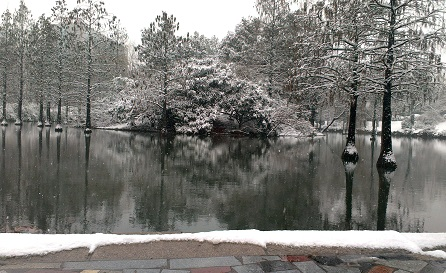
\includegraphics[width=0.7\textwidth]
  {IMAG1546.jpg}

图:中国科学技术大学西校区-也西湖雪景

拍摄于2015.1.28 - 11:30
\end{figure}

本课程参考以下教材:

1. \verb"Demailly: Complex analytic and differential geometry."

2.  \verb"Huybrechts: Complex geometry: an introduction."

3.  \verb"Morrow, Kodaira: Complex manifolds."

4. \verb"Grauert, Remmert: Coherent analytic sheaves."

5. \verb"Hormander: An introduction to complex analysis in several variables."

6. \verb"Griffiths, Harris: Principles of algebraic geometry."

\fengexian

\begin{center}
在五道口也要红专并进、理实交融呀$\sim$
\end{center}

\tableofcontents
\chapter{多复变函数}
%应该补充一些复线性空间的线性代数,单独构成一节。
\section{多元全纯函数}
首先快速回顾单复变函数的知识。
我们通常用$\Omg$来表示$\bbC$的开子集,
$z=x+iy$为$\bbC$的坐标。对于$z\in\bbC$以及实数$R>0$,我们令
$$\bbD(z,R):=\{w\in\bbC|\,|w-z|< R\}$$
为以$z$为圆心$R$为半径的开圆盘。

此外,我们有如下常用记号:
$$\left\{\begin{array}{l}
\td z:=\td x + i\td y\\
\td \bar{z} := \td x- i\td y
\end{array}\right.\quad
\left\{\begin{array}{l}
\pp{z}:=\frac{1}{2}
\left(\pp{x}-i\pp{y}\right)\\
\pp{\bar{z}} := \frac{1}{2}
\left(\pp{x}+i\pp{y}\right)
\end{array}\right.
$$
对于函数$f:\Omg\to\bbC$,
称$f$是\textbf{全纯}(holomorphic)的,
\index{holomorphic function\kong 全纯函数}
若在$\Omg$中成立
$$\pbar f:=\pfrac{f}{\bar{z}}\td\zbar=0$$
我们知道,$f$是全纯的当且仅当$f$在$\Omg$
处处能够局部地展开为收敛幂级数。

对于$\bbC$中的紧致集$K$,称函数$f:K\to\bbC$是全纯的,
如果存在$K$的开邻域$\Omg\supseteq K$,
使得$f$可延拓为$\Omg$上的全纯函数。

单复变函数论中有如下重要结果:

\begin{thm}(柯西积分公式)
设$\bbD\subseteq\bbC$为$\bbC$中的开圆盘,$f:\bbD\to\bbC$为
$\bbD$上的全纯函数,且在$\p\bbD$连续,
则对于任意$w\in\bbD$,成立
$$f(w)=\frac{1}{2\pi i}\int_{\p\bbD}\frac{f(z)}{z-w}\td z$$
\end{thm}

此定理能推导出单变量全纯函数理论的“almost everything”.
这里不再赘述。

我们开始考虑多变量全纯函数。

\begin{definition}
设$\Omg\subseteq\bbC^n$为$\bbC^n$的开子集,函数$f:\Omg\to\bbC$
称为(多变量)\textbf{全纯函数},如果满足以下条件:

(1)$f$是连续函数;

(2)对任意$1\leq j\leq n$,以及任意固定的
$z_1,...,z_{j-1};z_{j+1},...,z_n\in\bbC$,关于$z_j$的单变量函数
$$z_j\mapsto f(z_1,...,z_{j-1};z_j;z_{j+1},...,z_n)$$
是(单变量)全纯函数。
\end{definition}

事实上,如果该定义中的(2)成立,那么能推出(1)成立,
也就是说此定义中的(1)可以去掉。其证明比较复杂,我们承认之。

\begin{notation}
对于$\bbC^n$的开子集$\Omg$,我们记
$$\mcalO(\Omg):=\{f:\Omg\to\bbC|f\text{是$\Omg$上的全纯函数}\}$$
\end{notation}
容易知道$\mcalO(\Omg)$有显然的$\bbC$-代数结构。\vs

本节将说明,多变量全纯函数具有一些与单变量全纯函数类似的性质。

\begin{notation}
对于$z=(z_1,z_2,...,z_n)\in\bbC^n$以及$R=(R_1,R_2,...,R_n)\in\bbR^n$,
并且$R_j>0\,\,(\forall 1\leq j\leq n)$,则我们记
$$\bbD(z,R):=\bbD(z_1,R_1)\times\bbD(z_2,R_2)\times
\cdots\times\bbD(z_n,R_n)$$
称为以$z$为中心,$R$为半径的\textbf{多圆柱}(polydisk)。
\index{polydisk\kong 多圆柱}

对于多圆柱$\bbD(z,R)$,我们记
$$\Gamma(z,R):=\p\bbD(z_1,R_1)\times\p\bbD(z_2,R_2)\times
\cdots\times\p\bbD(z_n,R_n)$$
称为$\bbD(z,R)$的\textbf{特征边界}(distinguished boundary)。
\index{distinguished boundary\kong 特征边界}
\end{notation}
特别注意特征边界$\Gamma(z,R)$
并不等于该多圆柱的边界$\p\bbD(z,R)$.

\begin{thm}(多变量全纯函数的柯西积分公式)

设$f:\overline{\bbD(z,R)}\to\bbC$为全纯函数,
则对任意的$w\in\bbD(z,R)$,成立
$$
  f(w)=
       \frac{1}{(2\pi i)^n}\int_{\Gamma(z,R)}
         \frac{f(\xi)\td\xi_1\td\xi_2\cdots\td\xi_n}
              {(\xi_1-w_1)(\xi_2-w_2)\cdots(\xi_n-w_n)}
$$
\end{thm}
\begin{proof}
由多变量全纯函数的定义,
反复使用单变量全纯函数的柯西积分公式即可。这是容易的。
\end{proof}

与单复变函数完全类似,我们也有泰勒展开:

\begin{cor}(多元全纯函数的泰勒展开公式)

对于$f\in\mcalO(\Omg)$,其中$\Omg\subseteq\bbC^n$为开子集,则
对于任何多圆柱$\bbD(z_0,R)$,如果
$\overline{\bbD(z_0,R)}\subseteq\Omg$,则对于任意$w\in\bbD(z_0,R)$,成立
$$
  f(w)=
       \sum_{\afa\in\bbN^n}a_\afa(w-z_0)^\afa
$$
其中
$$
  a_\afa=\frac{1}{(2\pi i)^n}
           \int_{\Gamma(z_0,R)}
             \frac{f(z)}
                  {(z-z_0)^{\afa+1}}
           \td z_1\td z_2\cdots\td z_n
  =\frac{f^{(\afa)}(z_0)}{\afa!}
$$
\label{多元泰勒-cor}
\end{cor}
注意这里的$\afa$为多重指标,即$\afa=(\afa_1,...,\afa_n)$,
其中每个$\afa_i$都为非负整数。
我们记
\begin{eqnarray*}
z^{\afa}&:=&z_1^{\afa_1}z_2^{\afa_2}\cdots z_n^{\afa_n}\\
\afa!&:=&\afa_1!\afa_2!\cdots\afa_n!\\
f^{(\afa)}&:=&(\p_{z_1})^{\afa_1}(\p_{z_2})^{\afa_2}\cdots(\p_{z_n})^{\afa_n}f\\
\afa+1&:=&(\afa_1+1,\afa_2+1,...,\afa_n+1)
\end{eqnarray*}

其中$z=(z_1,...,z_n)\in\bbC^n$,$f$为$n$元全纯函数。
\begin{proof}
与单复变函数的情形完全类似,可由柯西积分公式得到。
\end{proof}

\begin{thm}(柯西不等式)对于$\bbC^n$的开子集$\Omg$,
若$f\in\mcalO(\Omg)$,多圆柱$\overline{\bbD(z_0,R)}\subseteq\Omg$,
则对任意多重指标$\afa\in\bbN^n$,成立
$$\left|f^{(\afa)}(z_0)\right|\leq
\frac{\afa!}{R^\afa}
\sup_{z\in\Gamma(z_0,R)}|f(z)|$$
\end{thm}
\begin{proof}
与单复变函数的情形完全类似。
利用多元泰勒展开(推论\ref{多元泰勒-cor})即可。
\end{proof}

\begin{cor}设$\Omg\subseteq \bbC^n$为\textbf{连通}开集,
$f\in\mcalO(\Omg)$满足$\forall 1\leq k\leq n$,
$\pfrac{f}{z_k}$在$\Omg$上恒为$0$,则$f$在$\Omg$上为常值函数。
\end{cor}

\begin{cor}(刘维尔定理)
设$f\in\mcalO(\bbC^n)$,并且满足
$$|f(z)|\leq A(1+|z|)^B$$
其中$A,B$为正实数,那么$f$必为次数不超过$B$的多项式函数。
\end{cor}

这些性质于单变量全纯函数雷同,证明也是类似的。

\begin{cor}(Montel定理)

设$\Omg$为$\bbC^n$的开子集,则$\mcalO(\Omg)$
中的任何局部一致有界的全纯函数列都存在一致收敛的子列。
\end{cor}
\begin{proof}
仍类似于单复变全纯函数的情形。使用柯西积分公式,再配合
Arzela-Ascoli定理即可。从略。
\end{proof}

现在,简单介绍一些复的微分形式。对于$\bbC^n$,记其复坐标为
$(z_1,z_2,...,z_n)$;视$\bbC^n$为$2n$维实线性空间,
$$z_k=x_k+iy_k$$
从而引入
\begin{eqnarray*}
\td z_k&=&\td x_k+i\td y_k\qquad (1,0)\text{形式}\\
\td \zbar_k&=&\td x_k-i\td y_k\qquad (0,1)\text{形式}
\end{eqnarray*}

\begin{definition}($(p,q)$-形式)

设$\Omg$为$\bbC^n$的非空开集,则形如
$$u(z)=\sum_{|I|=p\atop |J|=q}
a_{IJ}(z)\td z_I\wedge\td\zbar_J$$
的光滑张量场称为$(p,q)$-形式。
记$\Omg$上的$(p,q)$-形式之全体为$C^\infty_{p,q}(\Omg)$.
\end{definition}
这里的$I,J$为多重指标。“光滑”指的是系数函数$a_{IJ}$为$\Omg$上的光滑复值函数。
另外,显然$(0,0)$-形式即为光滑函数;
$C^\infty_{p,q}(\Omg)$具有显然的复线性空间结构,
事实上还是$C^\infty(\Omg)$-模。

\begin{notation}($\pbar$-算子)
定义算子
$$\pbar: C^\infty_{p,q}(\Omg)\to C^\infty_{p,q+1}(\Omg)$$
如下:对于$(p,q)$-形式
$$u:=\sum_{|I|=p\atop|J|=q}
a_{IJ}\td z_I\wedge\td\zbar_J$$
则
$$
  \pbar u=
  \sum_{|I|=p\atop|J|=q}
    \sum_{k=1}^n
      \pfrac{a_{IJ}}{\zbar_k}
      \td \zbar_k\wedge\td z_I\wedge\td\zbar_J
$$
\end{notation}
类似地,也有
$$\p:C_{p,q}^\infty(\Omg)\to C_{p+1,q}^\infty(\Omg)$$
它们与外微分算子$\td$满足关系
$$\td=\p+\pbar$$
由$\td^2=0$,易知
$$\p^2=0,\quad \pbar^2=0,\quad \p\pbar+\pbar\p=0$$

以下事实显然成立:
\begin{lemma}
对于区域$\Omg$上的光滑函数$f\in C^\infty(\Omg)$,
则$f$全纯当且仅当$\pbar f=0$.
\end{lemma}

\begin{rem}(Dolbeault上同调)
对于$\Omg\subseteq\bbC^n$,注意$\pbar^2=0$,
从而对任意$p\geq 0$,有上链复形$C^\infty_{p,\bullet}(\Omg)$:
$$
  \cdots\to
  C^\infty_{p,q-1}(\Omg)
  \xra{\pbar}C^\infty_{p,q}(\Omg)
  \xra{\pbar}C^\infty_{p,q+1}(\Omg)
  \to\cdots
$$
称上同调群
$$H^{p,q}(\Omg):=H^q(C^\infty_{p,\bullet}(\Omg),\pbar)$$
为区域$\Omg$的\textbf{Dolbeault上同调群}。
\index{Dolbeault cohomology}
\end{rem}
类似于外微分$\td$的de-Rham上同调群,
Dolbeault上同调群与$\Omg$的拓扑联系密切。
例如,以下定理十分重要,我们先陈述,以后再证明:

\begin{lemma}(Dolbeault-Grothendieck引理)

设$\bbD\subseteq\bbC^n$为多圆柱,则对于任意$p,q\geq 0$,
$$H^{p,q}(\bbD)=0$$
\end{lemma}

不难发现它与de Rham上同调的Poincare引理有些类似。

\section{解析延拓与Hartogs现象}
上一节介绍了多复变函数的一些“普通的”(与单变量类似)性质,
本节开始介绍多复变函数的一些独特性质。

\begin{lemma}设$f\in C^\infty_c(\bbC)$为复平面上的
紧支光滑函数,则对任意$z\in\bbC$,成立
$$
  \frac{1}{2\pi i}
  \iint_\bbC
    \frac{\p f\big/\p\taubar}
         {\tau-z}
    \td\tau\wedge\td\taubar
=f(z)$$
\end{lemma}
\begin{proof}
基本的微积分练习。考虑换元$\tau=z+re^{i\theta}$,则易知
\begin{eqnarray*}
  \td\tau\wedge\td\taubar&=&-2ir\td r\wedge\td\theta\\
  \pfrac{r}{\taubar}&=&\frac{1}{2}e^{i\theta}\\
  \pfrac{\theta}{\taubar}&=&-\frac{1}{2ir}e^{i\theta}
\end{eqnarray*}
因此有
\begin{eqnarray*}
     \frac{1}{2\pi i}
     \iint_\bbC
       \frac{\p f\big/\p\taubar}
            {\tau-z}
       \td\tau\wedge\td\taubar
&=&
     \frac{-1}{2\pi}
       \int_0^\infty\td r
         \int_0^{2\pi}
           \left(
            -\frac{1}{ir}\pfrac{f}{\theta}(z+re^{i\theta})
           \right)
           \td\theta\\
& &
    +\frac{-1}{2\pi}
     \int_0^{2\pi}\td\theta
       \int_0^\infty
       \left(
         \pfrac{f}{r}(z+re^{i\theta})
       \right)
       \td r\\
&=&
     0+\frac{-1}{2\pi}
     \int_0^{2\pi}
       -f(z)
       \td\theta\\
&=&
     f(z)
\end{eqnarray*}
证毕。
\end{proof}

\begin{lemma}(简单版本的$\pbar$-引理)

设$n\geq 2$,$\fai\in C^\infty_{0,1}(\bbC^n)$
为具有紧支集的光滑$(0,1)$-形式,
且$\pbar\fai=0$,则存在$\bbC^n$上的紧支光滑函数$g$,使得
$$\pbar g=\fai$$
\label{partial-bar引理-简单版本-lemma}
\end{lemma}

\begin{proof}
记光滑$(0,1)$-形式$\fai$为
$$\fai=\sum_{k=1}^n\fai_k(z_1,...,z_n)\td\zbar_k$$
则
\begin{eqnarray*}
     \pbar\fai
&=&
     \sum_{k,l}
       \pfrac{\fai_k}{\zbar_l}
       \td\zbar_l\wedge\td\zbar_k
 =
     \sum_{1\leq l<k\leq n}
       \left(
         \pfrac{\fai_k}{\zbar_l}
        -\pfrac{\fai_l}{\zbar_k}
       \right)
       \td\zbar_l\wedge\td\zbar_k
\end{eqnarray*}
从而由$\pbar\fai=0$可得对任意$k\neq l$,
$$\pfrac{\fai_k}{\zbar_l}=\pfrac{\fai_l}{\zbar_k}$$

考虑如下的$\bbC^n$上的函数$\psi$:对于$z=(z_1,...,z_n)\in\bbC^n$,
$$
  \psi(z)
:=
  \frac{1}{2\pi i}
  \iint_\bbC
    \frac{\fai_1(\tau;z_2,...,z_n)}
         {\tau-z_1}
    \td\tau\wedge\td\taubar
$$
由$\fai_1$的紧支性易知$\psi$为$\bbC^n$上的光滑函数。
对于$1<k\leq n$,有
\begin{eqnarray*}
     \pfrac{\psi(z)}{\zbar_k}
&=&
     \frac{1}{2\pi i}
     \iint_\bbC
       \frac{\pfrac{\fai_1}{\zbar_k}(\tau;z_2,...,z_n)}
            {\tau-z_1}
       \td\tau\wedge\td\taubar\\
&=&
     \frac{1}{2\pi i}
     \iint_\bbC
       \frac{\pfrac{\fai_k}{\taubar}(\tau;z_2,...,z_n)}
            {\tau-z_1}
       \td\tau\wedge\td\taubar\\
&=&
    \fai_k(z)
\end{eqnarray*}
上式对$k=1$显然也成立。因此$\pbar\psi=\fai$.

最后还需要证明$\psi$是紧支的。
由于$\fai$紧支,存在足够大的$R>0$,使得
$$\supp\fai\subseteq \bbD(0,R)$$
因此任意取定$z\in\bbC^n$,使得$z$的分量$z_2,z_3,...,z_n$之中
至少有一个模长大于$R$,则由$\psi$的定义式直接得到$\psi(z)=0$.
(注意:这一步严重依赖$n\geq 2$!)也就是说,存在$z\not\in\bbD(0,R)$
使得$\psi=0$在$z$的某邻域内都成立。
另一方面,由于$\pbar\psi=\fai$且$\supp\fai\subseteq\bbD(0,R)$,
从而$\psi$在$\bbD(0,\bbR)$外部全纯,因此由解析延拓唯一性,
$\psi$在$\bbD(0,R)$外部恒为零,因此$\psi$紧支。
\end{proof}

此引理在单复变$n=1$的情形\textbf{不成立}:
\begin{example}
设$\fai_1\in C_0^\infty(\bbC)$为复平面上的紧支光滑函数,并且
$$\iint_\bbC\fai_1(z)\neq 0$$
考虑$\bbC$上的$(0,1)$-形式$\fai=\fai_1(z)\td\zbar$,
则$\pbar\fai=0$是平凡的,
但\textbf{不存在}紧支光滑函数$\psi$使得$\pbar\psi=\fai$.
\end{example}

\begin{proof}
若存在紧支光滑函数$\psi$使得$\pbar\psi=\fai$,
则$\pfrac{\psi}{\zbar}=\fai_1$.于是
$$
  0\neq
  \iint_\bbC
    \fai_1(z)\td z\wedge\td\zbar
=
  \iint_\bbC
    \pfrac{\psi}{\zbar}
    \td z\wedge\td\zbar
=0
$$
产生矛盾。
\end{proof}

以下是多复变函数解析延拓的令人惊讶的性质,
它与单复变函数有本质不同:

\begin{thm}(Hartogs现象)

设$\Omg\subseteq\bbC^n$为开集$(n\geq 2)$,
$K\ssubset\Omg$且为$\bbC^n$的紧子集,
则对任意的$f\in\mcalO(\Omg\setminus K)$,
都存在解析延拓$F\in\mcalO(\Omg)$,使得
$$F|_{\Omg\setminus K}=f$$
\end{thm}

\begin{proof}
取$K$与$\Omg$直接的截断函数$\psi\in C^\infty_0(\bbC^n)$,
使得$0\leq \psi\leq 1$,
$$K\ssubset\supp\psi\ssubset\Omg$$
并且$\psi|_K\equiv 1$.
考虑$$\ftil:=(1-\psi)f$$
则$\ftil$在整个$\Omg$上都有定义。注意
$$\pbar\ftil=-(\pbar\psi)f+(1-\psi)\pbar f$$
易知$\supp\pbar\ftil\subseteq\supp\psi$.于是由
引理\ref{partial-bar引理-简单版本-lemma},存在光滑函数
$v$,使得$\supp v\subseteq\psi$,并且$\pbar v=\pbar\ftil$,
从而考虑函数
$$F:=(1-\psi)f-v$$
则$\pbar F=0$,从而$F\in\mcalO(\Omg)$.又因为易知
$$F=f\quad(\forall z\in\Omg\setminus\supp\psi)$$
从而由解析延拓唯一性,有$F_{\Omg\setminus K}=f$.
\end{proof}

关于解析延拓,再介绍如下结果:

\begin{lemma}(Hartogs figure)
\index{Hartogs figure}

对于$n>1$,正实数$0\leq r<R$,
以及$\bbC^{n-1}$的开子集$\omg'\subseteq\omg$,
其中$\omg$是连通的。记$\bbC^n$的开子集
$$
  \Omg:=
    \left(
      (\bbD(0,R)\setminus\bbD(0,r))\times\omg
    \right)
    \cup
    \left(
      \bbD(0,R)\times\omg'
    \right)
$$
其中$\bbD(0,r)$与$\bbD(0,R)$
分别为$\bbC$上的以原点为中心,$r,R$为半径的开圆盘。
则任意$f\in\mcalO(\Omg)$都可以(唯一地)解析延拓至
$$\widetilde{\Omg}:=\bbD(0,R)\times\omg$$
\end{lemma}
如此的区域$\Omg$称之为“\textbf{Hartogs figure}”。
$\Omg$的几何图像大致如下:

\begin{figure}[ht]
\centering
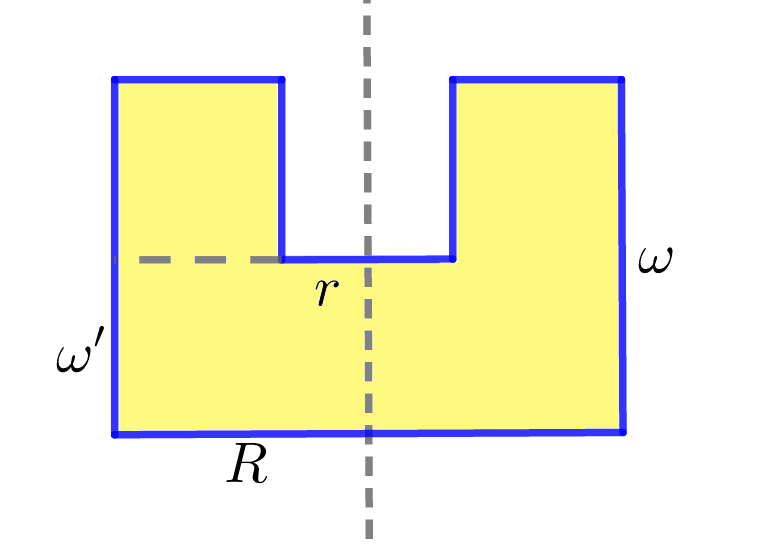
\includegraphics[width=0.4\textwidth]
  {figures/HartogsFigure.png}

图:Hartogs figure示意
\end{figure}

\begin{proof}
容易知道
$$\Omg=\big\{(z_1,\ztil)\in\bbC\times\bbC^{n-1}\big|
r<|z_1|<R,\ztil\in\omg\text{或者}
|z_1|\leq r,\ztil\in\omg'
\big\}$$
对于$f\in\mcalO(\Omg)$,定义$\Omgtil$上的函数
$$
  \ftil(z_1,\ztil):=
    \frac{1}{2\pi i}
    \int_{|w|=\rho}
      \frac{f(w,\ztil)}
           {z_1-w}
      \td w
$$
其中$\rho$为满足$\max\{r,|z_1|\}<\rho<R$的任意实数。
则易知如此定义的$\ftil$为$f$在$\Omgtil$上的解析延拓。
\end{proof}

\begin{thm}(Riemann延拓定理)

考虑$\bbC^n$中的多圆柱$\bbD(0,R)$,其中$n\geq 2$,$R\in\bbR_+^n$。
对任意$2\leq p\leq n$,令$\bbC^n$的子集
$$S:={(z_1,...,z_n)\in\bbC^n|z_1=\cdots=z_p=0}$$
则对任意$f\in\mcalO(\bbD(0,R)\setminus S)$,
$f$都可(唯一地)解析延拓至$\bbD(0,R)$.
\end{thm}

\begin{proof}
这是Hartogs figure的显然推论。记$R=(R_1,R_2,...,R_n)$,
以及$R':=(R_2,...,R_n)\in\bbR^{n-1}$.
考虑$\bbC^{n-1}$的开子集
\begin{eqnarray*}
  \omg &:=&\bbD(0,R')\\
  \omg'&:=&\omg\setminus\{z_2=\cdots=z_p=0\}
\end{eqnarray*}
则易知
$$\bbD(0,R)\setminus S=
\Big(
  \bbD(0,R_1)\setminus\{0\}\times\omg
\Big)
\cup
\Big(
  \bbD(0,R_1)\times\omg'
\Big)
$$
为Hartogs figure,从而完。
\end{proof}

\section{Weierstrass预备定理与除法定理}
(待补)







%%%%%%%%%%%%%%%%%%%%%%%%%%%%%%%%%%%%%%%%%%%%%%%%%
%%%%%%%%%%%%%%%%%%%%%%%%%%%%%%%%%%%%%%%%%%%%%%%%%
%       2019.3.21启用电子稿                     %
%%%%%%%%%%%%%%%%%%%%%%%%%%%%%%%%%%%%%%%%%%%%%%%%%

\chapter{层与层上同调}
\section{层的上同调}
Today:

Sheaf cohomology

$X$ a topological space, $\mcalF$- sheaf (of abelian groups).

\begin{definition}  (resolution)

(1)a resolution of $\mcalF$ is an exact sequence

$$0\to \mcalF\xra{j}\mcalF\xra{d^0}\mcalF\xra{d^1}\to\cdots$$

\end{definition}

\begin{definition}
A sheaf $\mcalA$ is called injective, if
if for any injective morphism $j:\mcalA\to \mcalB$
and for any morphism $\fai:\mcalA\to\mcalS$,
there exists an extension $\psi :\mcalB\to \mcalS$,such that
%%%%%diagram%%%
\end{definition}
\begin{thm}
the category of sheaves of abelian sheaves have enough
injective objects, i.e.  any $\mcalF$ can be
embedded in some injective sheaf.
\end{thm}

\begin{definition}
Consider an injective resolution of $\mcalF$, i.e. an exact sequence
$$0\to\mcalF\to\mcalI^0\xra{\td}\mcalI^1\xra{\td}\mcalI^2\to\cdots$$
where every $\mcalI^k(k\geq 0)$ is injective.


$\rightsquigarrow $induces a sequence
$$0\to\Gamma(X,\mcalF)
\to\Gamma(X,\mcalI^0)\xra{\td}
\Gamma(X,\mcalI^1)\xra{\td}
\Gamma(X,\mcalI^2)\to\cdots$$

Then
$$H^q(X,\mcalF):=H^q(\Gamma(X,\mcalI\updot))$$

\end{definition}

then, $H^0(X,\mcalF)=\Gamma(X,\mcalF)$.

\begin{definition}
A sheaf $\mcalS$ is called a flabby (flasque ,in France) ,if
for any open set $\Omg\subseteq X$, the morphism
$$\mcalS(X)\to\mcalS(\Omg)$$
is surjective.
\end{definition}

\begin{definition}
$$0\to\mcalF\xra{j}\mcalF^0\xra{d^0}\to\mcalF^1$$
is an exact sequence is called a flabby resolution, if
any $\mcalF^k$ is flabby.
\end{definition}

\begin{definition}
$$H^q(X,\mcalF):=...\text{by flabby resolution...}$$
\end{definition}

\begin{proof}
Homological Algebra...omit.
\end{proof}

the two definitions of Sheaf Cohomology are isomorphic.


Godement's construction

$$God(\mcalF)(U):=
\{f:U\to\bigcup_{x\in U}\mcalF_x|
f(y)\in\mcalF_y,\forall y\in U\}
:=\prod_{x\in U}\mcalF_x$$

$God(\mcalF)$ is a sheaf, and it is flabby. and there is a canonical
morphism $\mcalF(U)\to God(F)(U)$ by $x\mapsto(x\mapsto s_x)$ is injective.

$$\mcalF^0:=God(\mcalF)$$
$$0\to\mcalF\xra{j}\mcalF^0\surj\coker(j)=\mcalF^0\big/\mcalF$$
and consider
$$\mcalF^1:=God(\coker(j))$$
......then construct by induction... this is a flabby resolution of $\mcalF$.

\begin{definition}(resolution by fine sheaves)

$\mcalA$ is a sheaf of ring,
$X$ is a paracompact topological space, $\mcalA$
is called a fine sheaf, if for any open covering
$$X=\bigcup_{\alpha}V_{\alpha}\quad,\mcalV:=\{V_{\alpha}\}$$
there exists a partition of unit subordinate to $\mcalV$,
(i.e. $\exists f_{\alpha}\in\mcalA(V_{\alpha}),supp(\alpha)
:=\overline{\{x\in V_{\alpha}|f_{\alpha,x}\neq 0\}}\subseteq V_{\alpha}$, and
$\sum_{\alpha}f_{\alpha}=1$(the sum is locally finite)
 )
\end{definition}

\begin{example}
$X$ is a differential manifold,
$\mcalC^{\infty}$ is the sheaf of smooth functions,
then $\mcalC^{\infty}$ is a fine sheaf.
\end{example}

\begin{thm}
$\mcalS$ is a sheaf of $\mcalA$-modules,
$\mcalA$ is a fine sheaf. then for any $q\geq 1$,
$$H^q(X,\mcalS)=0$$
\end{thm}
\begin{proof}
Consider a flabby(or injective) resolution
$$0\to\mcalS\xra{j}\mcalI^0\xra{\td}\mcalI^1\xra{\td}\mcalI^2\cdots$$
where any $\mcalI^k(k\geq 0)$ is a sheaf of $\mcalA$-modules.

by definition,
$$H^q(X,m\mcalS):=\frac{\ker\td:\Gamma(\mcalI^q)\to\Gamma(\mcalI^{q+1})}
                       {\Im\td:\Gamma(\mcalI^{q-1})\to\Gamma(\mcalI^{q})}$$

Let $\alpha\in\ker\{\td:\Gamma(\mcalI^q)\to\Gamma(\mcalI^{q+1})\}$
by the exactness of resolution, $\exists$ an open covering $\mcalU=(U_{i})_{i}$,
s.t. $\alpha|_{U_{i}}=\td\beta_{i}$
where $\beta_{i}\in\mcalT^{q-1}(U_{i})$.
Let $(\beta_{i})_{i}$ be the partition of unit w.r.t. $\mcalU$.
consider
$$\beta:=\sum_{i}f_i\beta_i$$
(well defined). Then $\td\beta=\alpha$....
\end{proof}

\section{\u{C}ech上同调}
\textbf{\u{C}ech cohomology}

$X$- a topological space, $\mcalF$- a sheaf of abelian group.
$$\mcalU=(U_{\alpha})_{\alpha\in I}$$
is an open covering.

notation:$U_{\alpha_1,...,\alpha_q}:=\bigcap_{i=1}^qU_{\alpha_i}$.

\u{C}ech $q$-chain w.r.t $\mcalU$:

$$C^q(\mcalU,\mcalF):=\prod_{(\alpha_1,...,\alpha_q)
\in\mcalI^{q+1}}\mcalF(U_{\alpha_1,...,\alpha_q})$$

$$c\in C^q(\mcalU,\mcalF)$$
means that we have a family of sections
$C_{\alpha_1,...,\alpha_q}\in\mcalF(U_{\alpha_1,...,\alpha_q})$
with the relation
$$C_{\alpha_0,...,\alpha_j,...,\alpha_i,...}=-C_{...}$$

\u(C)ech differential:
$$\delta^q:C^q(\mcalU,\mcalF)\to C^{q+1}(\mcalU,\mcalF)$$
$$\delta^q(c)_{\alpha_0,...,\alpha_{q+1}}
:=\sum_{0\leq k\leq q+1}(-1)^k
c_{...\hat{\alpha_k}...}|_{U_{\alpha_0,...,\alpha_{q+1}}}$$

\begin{prop}
$$\delta^q\circ\delta^q=0$$
\end{prop}

so, we have \u{C}ech cohomology
$$H^q(\mcalU,\mcalF):=\ker\delta^q\big/\im\delta^{q-1}$$

example:
$$C^0(\mcalU,\mcalF):=\prod_{\alpha\in I}\mcalF(U_{\alpha})$$
$$c=(c_{\alpha})_{\alpha\in I}\in C^0(\mcalU,\mcalF)$$
$$\delta^0c=0\iff(\delta^0c)_{\alpha_0\alpha_1}
:=(c_{\alpha_1}-c_{\alpha_0})|_{U_{\alpha_0\alpha_1}}=0$$
so, $c_{\alpha_0}=c_{\alpha_1}$ on $U_{\alpha_0\alpha_1}$.

$\rightsquigarrow$ $H^0(\mcalU,\mcalF)=\mcalF(X)$.

\begin{example}
(1) consider $X=\triangle\setminus\{0\}$, where $\triangle=
\{(z_1,z_2)||z_1|<1,|z_2|<1\}$. Consider the covering
$$\mcalU=U_1\cup U_2$$
where
$$U_1:=\{(z_1,z_2)\in\triangle|z_1\neq 0\}=\bbD^*\times\bbD$$
$$U_2:=\{(z_1,z_2)\in\triangle|z_2\neq 0\}=\bbD\times\bbD^*$$

then
$$U_1\cap U_2=\bbD^*\times\bbD^*$$

consider $H^0(X,\mcalO)=\mcalO(X)\cong\mcalO(\triangle)
=\{f:\triangle\to\bbC\text{holomorphic}\}$.

$$H^1(\mcalU,\mcalO)=\ker\delta^1\big/\im\delta^0$$
$$\delta^1:C^1(\mcalU,\mcalO)\to C^2(\mcalU,\mcalO)\subseteq
\prod_{\alpha_0,\alpha_1,\alpha_2}\mcalO(U_{\alpha_0,\alpha_1,\alpha_2})=0$$
$$\ker\delta^1=
C^1(\mcalU,\mcalO)=\{c=c(\alpha_0,\alpha_1)|c_{\alpha_0,\alpha_1}\in\mcalO(U_{\alpha_0\alpha_1})\}
=\{c\in\mcalO(U_1\cap U_2)\}=\{c=\sum_{m,n\in\bbZ}a_{mn}z_1^mz_2^n\text{convergent}\}$$

$$\delta^0:C^0(\mcalU,\mcalO)\to\mcalC^1(\mcalU,\mcalO)$$
$$(\delta^0c)_{12}=(c_2-c_1)|_{U_{12}}$$
where $c_2\in\mcalO(U_2)$ and $c_1\in\mcalO(U_1)$.
note that
$$\mcalO(U_1)=\{c(z_1,z_2)=\sum_{m\in\bbZ,n\geq 0}a_{mn}z_1^mz_2^n\text{convergent}\}$$
$$\mcalO(U_2)=\{c(z_1,z_2)=\sum_{n\in\bbZ,m\geq 0}a_{mn}z_1^mz_2^n\text{convergent}\}$$

So, $H^1(\mcalU,\mcalO)=
\{c(z_1,z_2)=\sum_{m,n<0}a_{mn}z_1^mz_2^n\}$
\end{example}

\begin{example}(complex projective space)

$$\bbC P^n:=(\bbC^{n+1}\setminus\{0\})\big/\sim$$
$$(z_0,...,z_n)\sim\lmd(z_0,...,z_n)$$
for some $\lmd\in\bbC^*$.

$$\bbC P^n=\{[z_0,...,z_n]|\text{not all $z_k=0$},z_i\in\bbC\}
=\bigcup_{0\leq p\leq n}V_k$$
where
$$V_k=\{[z_0,...,z_n]|z_k\neq 0\}
\cong \{(\frac{z_0}{z_k},...,1,...,\frac{z_n}{z_k})|
z_i\in\bbC,i\neq k, z_k\neq 0\}\cong \bbC^n$$
this is a holo chart.

$$\bbC P^1=V_0\cup V_1,\mcalV=\{V_0,\mcalV_1\}$$
HW: compute $H^q(\mcalV,\mcalO)$.

Answer:
$$H^0\cong\bbC,H^1\cong 0$$
\end{example}

%%%%%%%%%%%%%%%%2019.3.26 第五周 周二%%%%%%%%%%%%%%%%%%%%%%%%%%%%%

\textbf{Correction}:

$\mcalA$: Sheaf of rings (with unit)

$X$: paracompact topological space,

\begin{definition}
$\mcalA$ is called fine, if for any open covering
$\mcalU=(V_{\alpha})_{\alpha\in\mcalI}$,there exist
$s_{\alpha}\in\mcalA(X)$
such that such that $supp(s_{\alpha})\subseteq V_{\alpha}$,
$$\sum_{\alpha}s_{\alpha}=1$$
(this is a locally finite sum)
\end{definition}

\begin{rem}
we call $\mcalA$ is a \textbf{soft sheaf},
if for any closed set $K\subseteq X$,
the morphism
$$\mcalA(X)\to \mcalA(K)$$
is surjective.
where $\mcalA(K):=\Gamma(K,\mcalA|_K)$
\end{rem}

fact: $\mcalA$ is fine if and only if
$\mcalH om(\mcalA,\mcalA)$ is soft.
(omit)

Recall:

Cech cohomology: $X$ topological space,
$\mcalU=(U_{\alpha})_{\alpha\in\mcalI}$,
$$C^q(\mcalU,\mcalF)=
\prod_{\alpha_0<...<\alpha_q}\mcalF(\U_{\alpha_1,...,\alpha_q})$$
$$\delta^q:C^q(\mcalU,\mcalF)\to C^{q+1}(\mcalU,\mcalF)$$

fact: $H^0(\mcalU,\mcalF)=\Gamma(X,\mcalF)$.

Today:

\begin{definition}
Let $\mcalV=(V_{\beta})_{\beta\in J}$ be another open covering,
then $\mcalV$ is called a refinement of $\mcalU$, if there exists a map
$$\rho:\mcalJ\to\mcalI$$
such that
$$V_{\beta}\subseteq U_{\rho(\beta)}$$
\end{definition}

\begin{prop}
Let $\mcalV$ be a refinement of $\mcalU$, then $\rho$ induces a map
$$\rho^q:C^q(\mcalU,\mcalF)\to C^q(\mcalV,\mcalF)$$
$$(\rho^qC)_{\beta_0,...,\beta_q}\mapsto
C_{\rho(\beta_0),...,\rho(\beta_q)}|_{V_{\beta_0,...,\beta_q}}$$
$\rho$ is a morphism of complexes.
\end{prop}

%%%%%%改用电子版了%%%%%%
so, $\rho$ induces a map
$$H^q(\rho):H^q(\mcalU,\mcalF)\to H^q(\mcalV,\mcalF)$$

Let $\tilde{\rho}:\mcalJ\to\mcalI$ be another refinement of $\mcalU$

(induces $H^q(\tilde{\rho}):H^q(\mcalU,\mcalF)\to H^q(\mcalV,\mcalF)$)
then $\rho,\tilde{\rho}$ are homotopic
%%%homotopy%%%
(chain homotopy$\rightsquigarrow H^q(\rho)=H^q(\tilde(\rho))$)

so, if $\rho:\mcalJ\to \mcalI$ is refinement, then
$$H^q(\rho)$$
is independent of the refinement.

\begin{definition}
$$\check{H}^q(X,\mcalF):=\lim_{\to\atop\mcalU} H^q(\mcalU,\mcalF)$$
i.e. $a\in H^q(\mcalU,\mcalF)\sim\in H^q(\mcalV,\mcalF)$ iff
$\exists$ a refinement $\mcalW$ of $\mcalU$ and $\mcalV$ such that
$a,b$ have the same image in $H^q(\mcalW,\mcalF)$
\end{definition}

\begin{rem}
$$\check{H}^0(X,\mcalF)=\Gamma(X,\mcalF)$$

Exercise: For $q=1$, if $\mcalV$ is a refinement of $\mcalU$,
then
$$H^1(\mcalU,\mcalF)\to H^1(\mcalV,\mcalF)$$
is injective.
\end{rem}

so ,for any open cover $\mcalU$,
$$H^1(\mcalU,\mcalF)\to \check{H}^1(X,\mcalF)$$
is injective.

\textbf{Homological Algebra}
recall:let $(K\updot,\td_k),(L\updot,\td_l)$ and $(M\updot,\td_M)$,
if we have a short exact sequence
$$0\to K\updot\xra{\fai} L\updot\xra{\psi}M\updot\to 0$$
then it induces a long exact sequence :
$$
  \cdots\to H^q(K\updot)\to
  H^q(L\updot)\to
  H^q(M\updot)\to
  H^{q+1}(K\updot)\to\cdots
$$

analogy of Cech cohomology: $X$ is a topological space,
$\mcalU$ is an open covering of $X$.
$\mcalA$ and $\mcalB$ sheaves on $X$, Let
$$\fai:\mcalA\to\mcalB$$
be a morphism, then it induces
$$\fai\updot:C\updot(\mcalU,\mcalA)\to C\updot(\mcalU,\mcalB)$$

Let
$$0\to \mcalA\to\mcalB\to\mcalC\to 0$$
be an exact sequence of sheaves, then we have:
for any open set $\Omg$,
$$0\to \mcalA(\Omg)\to \mcalB(\Omg)\to\mcalC(\Omg)$$
left exact.

Example: consider
$$0\to\bbZ\to\mcalO\xra{exp}\to0$$
is exact on $bbC^{\times}:=\bbC\setminus\{0\}$

but we have :
$$0\to\mcalA(\Omg)\xra{\psi}\mcalB(\Omg)\to\im\psi(\Omg)\to 0$$
is exact.

First we have the following exact sequence
$$C^q(\mcalU,\mcalA)\to C^q(\mcalU,\mcalB)\to C^q_{\mcalB}(\mcalU,\mcalC)\to 0$$
where $C_{\mcalB}^q$ is the image of ...

then we get an exact sequence
$$0\to (C\updot(\mcalU,\mcalA),\delta)\to
(C\updot(\mcalU,\mcalB),\delta)\to
(C\updot_{\mcalB}(\mcalU,\mcalC),\delta)\to 0$$

it induces a long exact sequence
$$\cdots\to
H^q(\mcalU,\mcalA)\to
H^q(\mcalU,\mcalB)\to
H^q_{\mcalB}(\mcalU,\mcalC)\to
H^{q+1}(\mcalU,\mcalA)\to\cdots
$$

\begin{thm}
If $X$ is paracompact,
$$0\to\mcalA\to\mcalB\to\mcalC\to 0$$
is a sheaf exact sequence.
Then there is a long exact sequence
$$
\cdots\to
\check{H}^q(X,\mcalA)\to
\check{H}^q(X,\mcalB)\to
\check{H}^q(X,\mcalC)\to
\check{H}^{q+1}(X,\mcalZ)\to \cdots
$$
\end{thm}
\begin{proof}

Key lemma: need to prove
$$\lim_{\to\atop\mcalU}H^q(\mcalU,\mcalC)=
\lim_{\to\atop\mcalU}H^q_{\mcalB}(\mcalU,\mcalC)
$$
if $X$ is paracompact.

Omit.
\end{proof}


if
$$0\to \mcalA\to\mcalB\to\mcalC\to 0$$
exact,

recall:(cohomology by resolutions)
$$
0\to\mcalA\to\mcalF^0\to\mcalF^1\to\cdots
$$
flabby resolution. then it induces
$$0\to\Gamma(X,\mcalA)\to\Gamma(X,\mcalF^0)\to\Gamma(X,\mcalF^1)\to\cdots$$
then define the sheaf cohomology...

we have a long exact sequence
$$
\cdots\to H^q(X,\mcalA)\to H^q(X,\mcalB)\to H^q(X,\mcalC)\to H^{q+1}(X,\mcalA)\to\cdots
$$
it is homological algebra...

\begin{thm}(Leray's acyclic theorem)
Let $\mcalU=(U_{\alpha})_{\alpha\in\mcalI}$ be an open covering of $X$,
($\mcalF$ is a sheaf on $X$), if satisfying
$$H^k(U_{\alpha_0,...,\alpha_q})=0$$
for any $k \geq 1$ ,then
$$H^q(\mcalU,\mcalF)\cong \check(H)^q(X,\mcalF)$$

and if $X$ is paracompact ,we also have
$$H^q(\mcalU,\mcalF)\cong \check(H)^q(X,\mcalF)\cong H^q(X,\mcalF)$$

\end{thm}
(this $\mcalU$ is called acyclic covering)

\textbf{de Rham- Weil theorem}
\begin{definition}
$\mcalF$ is a sheaf on $X$, $\Omg$ is an open set of $X$,
then $\mcalF$ is called \textbf{acyclic sheaf} if
$$H^q(\Omg,\mcalF)=0$$
for any $q\geq 1$.
\end{definition}

\begin{thm}
Let
$$0\to\mcalF\to(L\updot,\td)$$
be an acyclic resolution of $\mcalF$
(i.e. $L^q$is acyclic on $X$)
then
$$H^q(X,\mcalF)\cong H^q(\Gamma(X,L\updot),\td)$$
for any $q\geq 0$.
\end{thm}

(先看例子)

\begin{example}
Let $X$ be a differential manifold,
$\mcalE^p$:sheaf of smooth $p$-forms, then we have a resolution
(de Rham complex)
$$0\to\bbR\inj\mcalE^0\xra{\td}\mcalE^1
\xra{\td}\mcalE^2\xra{\td}\mcalE^3\to\cdots$$
where $\td$ differential operators.
(Why it is a resolution? because of Poincare lemma...locally solvable..)

Note that
$$\mcalE^0=\mcalC^{\infty}$$
$\mcalE^p$ is a sheaf of $C^{\infty}$-modules..

then we have
$$H^q(X,\mcalE^p)=0$$
for all $q\geq1$

and then
$$H^q(X,\bbR)\cong
\frac{\ker(\td:\Gamma(X,\mcalE^q)\to\Gamma(X,\mcalE^{q+1}))}
     {\im(\td:\Gamma(X,\mcalE^{q-1})\to\Gamma(X,\mcalE^q))}
=H_{DR}^q(X,\mcalR)
$$
\end{example}

\begin{example}
Let $X$ be a complex manifold,
$\mcalE^{p,q}$ sheaf of smooth $(p,q)$ forms,
$\Omg^p$ is the sheaf of holomorphic $p$-forms
(i.e. $(p,0)$-form $\fai$ with $\pbar\fai=0$).

Then we have resolution
$$0\to \Omg^p\xra{j}\mcalE^{p,0}\xra{\pbar}\mcalE^{p,1}\xra{\pbar}\mcalE^{p,2}\to\cdots$$
(Why it is a resolution?  because of the Dolbeault lemma),remain to Exercise...

$$H^q(X,\Omg^p)\cong H^{p,q}_{\pbar}(X,\bbC)$$
\end{example}

%%%%%%%%%%%%%%%%%2019.3.28第五周周四%%%%%%%%%%%%%%%%%%%%%%%%%

Today: de Rham-Weil Isomorphism Thm

\begin{thm}
Let $X$ be a topological space, $\mcalF$ be a sheaf of abelian groups on $X$,
$$0\to\mcalF\to(\mcalL\updot,\td)$$
be an acyclic resolution, i.e.
$$H^k(X,\mcalL^q)=0$$
for all $k\geq 1$ and $q\geq 0$.
Then,
$$H^q(X,\mcalF)\cong H^q((\Gamma(\mcalL\updot),\td))$$
\end{thm}

\begin{proof}
Since
$$
0\to \mcalF\xra{j}\mcalL^0\xra{\td^0}\mcalL^1\xra{\td^1}\mcalL^2\to\cdots
$$
be an exact sequence, denote
$$\mcalZ^q:=\ker \td^q$$
then we have short exact sequences
$$0\to \mcalZ^q\to\mcalL^q\to\mcalZ^{q+1}\to 0$$
for any $q$. They induce long exact sequence of cohomology groups:
$$\cdots\to H^k(X,\mcalZ^q)\to H^k(X,\mcalL^q)\to H^k(X,\mcalZ^{q+1})\xra{\p}
H^{k+1}(X,\mcalL^q)\to H^{q+1}(X,\mcalL^q)\to\cdots$$
For any $k\geq 1$, since $\mcalL^q$ are acyclic on $X$,
$$H^k(X,\mcalZ^{q+1})\cong H^{k+1}(X,\mcalZ^q)$$
and for $k=0$, we have
$$
0\to H^0(X,\mcalZ^q)\to H^0(X,\mcalL^q)\to H^0(X,\mcalZ^{q+1})\to
H^1(X,\mcalZ^q)\to H^1(X,\mcalL^q)=0\to\cdots
$$
so,
$$H^1(X,\mcalZ^q)\cong H^0(X,\mcalZ^{q+1})\big/\im\td^q
\cong H^{q+1}((\Gamma(\mcalL\updot),\td))$$

$$H^{q+1}(\Gamma(\mcalL\updot))\cong H^1(X,\mcalZ^q)\cong H^2(X,\mcalZ^{q-1})\cong\cdots
H^{q+1}(X,\mcalZ^0)=H^{q+1}(X,\mcalF)$$
\end{proof}

%%%%%%%上次课讲了两个经典例子:De Rham cohomology and Doulbeault cohomology%%%%%%55

$$0\to\bbR\to\mcalE^0\xra{\td}\mcalE^1\xra{\td}\mcalE^2\to\cdots$$
(de Rham resolution) then we have
$$H^k(X,\mcalR)\cong H_{DR}^k(X;\mcalR)$$
(if $X$ is compact ,then by Hodge theory, it also isomorphic to $\ker(\td\td^*+\td^*\td)$)

Another example:$X$ is a complex manifold, then
$$0\to\Omg^p\to\mcalE^{p,0}\xra{\pbar}\mcalE^{p,1}\xra{\pbar}\mcalE^{p,2}\to\cdots$$
then
$$H^{q}(X,\Omg^p)\cong H_{\pbar}^{p,q}(X,\bbC)$$
(RHS$=$ Dolbeault cohomology)


$X$ be a smooth manifold, we define
$$C_q(X,\bbZ):=\text{the free abelian group generated by continuous map}$$
$$\phi:\triangle_q:=\{(t_1,...,t_{q+1})\in[0,1]^{q+1}|\sum_{i=1}^nt_i=1\}$$
and we define (for $\phi\in C_q(X,\bbZ)$)
$$\p\phi:=\sum_{i=1}^{q+1}(-1)^q\phi|_{\triangle_{q,i}}$$
$$\triangle_{q,i}:=\{t\in\triangle_q|t_i=0\}$$
we define
$$(C_{sing}\updot,\p)$$
be the dual complex of $(C^{sing}\downdot),\p$.

(These are all Basic Algebraic Topology)

For any open $U\subseteq X$, we have
$$U\to C_{sing}^q(U,\bbZ)$$
we get a sheaf
$$\mcalC_{sing}^q$$

FACT: $(\mcalC_{sing}\updot,\p)$ is a flabby resolution of $\bbZ$. (check!)So,
$$H^q_{sing}(X,\bbZ)= H^q(\Gamma(\mcalC_{sing}\updot),\p)
\cong H^q(X,\bbZ)$$

%%%%%%%%%%%%%%%以后还要讲谱序列,so scared...好怕怕……%%%%%%%%%%%%%%%%%%%5
%推荐读一读,现在学的东西应该能读懂了。。。
%Tate : rigid analytic spaces
%%%%%%%%%%%%%%%%%%%%%%%%%%%%%%%%%%%

\chapter{Hermite向量丛}
\section{联络与曲率}

Recall: $X$ is a smooth manifold, $E$ is a vector bundle of rank $r$, if

(1)$\pi:E\to X$ is smooth map,

(2)for any $x\in X$, $E_x:=\pi^{-1}(x)$ is a vector space over $\bbK$
($\bbK=\bbR$ or $\bbC$) of dimension $r$.

(3)there an open covering $\mcalU=(\mcalU_{\alpha})_{\alpha\in I}$ and trivializations
$$\theta_\alpha: E|_{U_{\alpha}}\cong U_{\alpha}\times \bbK^r$$
and for any intersection $U_{\alpha}\cap U_{\beta}$, we have
%%%%%%%见笔记%%%%%%%%%5

\begin{rem}
$$g_{\alpha\beta}=g_{\beta\alpha}^{-1}$$
$$g_{\alpha\beta}g_{\beta\gamma}g_{\gamma\alpha}=1$$
(cocycle condition)
\end{rem}

\textbf{Special Case: line bundle}
rank $E$=1.

then $g_{\alpha\beta}\in C^{\infty}(U_{\alpha\beta},\bbK^*)=\mcalE^*(U_{\alpha\beta})$
invertible smooth function on $U_{\alpha\beta}$.
then, Cech cohomology,
$$(\delta g)_{\alpha\beta\gamma}=g_{\beta\gamma}g_{\alpha\gamma}^{-1}g_{\alpha\beta}=1$$
so,
$$(g_{\alpha,\beta})\in\mcalZ^1(\mcalU,\mcalE^*)
\surj H^1(\mcalU,\mcalE^*)\inj\check{H}^1(X,\mcalE^*)$$
we get a map
$$\{\text{line bundles}\}\to \check{H}^1(X,\mcalE^*)$$
actually, we have
$$\{\text{isomorphic classes of line bundles}\}
\longleftrightarrow H^1(X,\mcalE^*)$$
1-1 correspondence.

Now, $X$ be a complex manifold,
a complex vector bundle $E$ is called homomorphic,
if ... the transition matrix $g_{\alpha\beta}$ is holomorphic...

Holomorphic line bundles :
$$g_{\alpha\beta}\in\mcalO^*(U_{\alpha\beta})$$
$\mcalO^*$:sheaf of invertible holomorphic functions...

FACT: there is a map
$$\{\text{holomorphic line bundle}\}\to\check{H}^1(X,\mcalO^*)$$

\begin{example}trivial vector bundle $X\times\bbK^r$
\end{example}

\begin{example}Tangent bundle $TX$.
(transition matrix $g_{\alpha\beta}$ are given by Jacobi matrix..)
\end{example}

\begin{definition}(Local frame of vector bundles)

$$\theta_{\alpha}:E|_{U_{\alpha}}\xra{\sim} U_{\alpha}\times\bbK^r$$
be a trivialization, we define
$$
  e_{\lmd}(x):=
  \theta_{\alpha}^{-1}
  (x,\begin{pmatrix}
       0\\
       \ldots\\
       1(\leftarrow i\text{th})\\
       \ldots\\
       0
     \end{pmatrix})
$$
then, $\{e_1,...,e_r\}$ be a local smooth section
$s\in\Gamma(U_{\alpha},E)$ can be written as
$$s(x)=\sum\sigma_{\lmd}(x)$$
where $\sigma_{\lmd}\in C^{\infty}(U_\alpha,\bbK)$.
\end{definition}

\textbf{(Connection)}

\begin{notation}

For $X$ be a smooth manifold, $E$ is a vector bundle(real or complex), denote
$$C_p^k(\Omg,E):=C^k(\Omg,\wedgeform{p}T^*M\ten E)$$
is the space of $k$-differential $p$-forms with values in $E$.

Locally, consider a trivialization of $E$,
$$\theta_{\alpha}E|_{U_{\alpha}}\cong U_{\alpha}\times \bbK^{r}$$
($\rightsquigarrow$ frame $(e_1,...e_r)$)
$$s\in \sum\fai_{\lmd}(x)\ten e_{\lmd}(x)$$
where $\fai_{\lmd}$ is a $p$-form.
\end{notation}

\begin{definition}
a (linear) connection on $E$ is a linear differential operator of order $1$ acting on
$C^{\infty}\downdot(X,E)$:
$$D:C_{p}^{\infty}(X,E)\to C_{p+1}^{\infty}(X,E)$$
$$D(f\wedge x):= \td f\wedge s+(-1)^p f\wedge Ds$$
where $f\in C^{\infty}(X,\wedgeform{p}T^*M)$, $s\in C^{\infty}(X,E)$.
\end{definition}

Locally, consider a local trivialization
$$\theta:E|_{\Omg}\xra{\sim}\Omg\times\bbK^r$$
with a frame $\{e_1,...,e_r\}$. any section
$t\in C^{\infty}_p(\Omg,E)$ can be written as
$$t=\sum_{1\leq\lmd\leq r}\sgm_{\lmd}\ten e_{\lmd}$$
$$Ds=\sum_{\lmd=1}^r\td\sgm_{\lmd}\wedge e_{\lmd}+(-1)^p\sgm_{\lmd}\wedge De_{\lmd}$$
where
$$De_{\lmd}\in C_1^{\infty}(\Omg, E)$$
can be written as
$$De_{\lmd}=\sum_{\mu=1}^r
             a_{\mu\lmd}\ten e_{\mu}$$
where "$a_{\mu \lmd}$" is called the coefficients of $D$
 with respect to frame $\{e_1,...,e_r\}$ .

so,
$$D(t)=
\sum_{\lmd,\mu}
  \td\sgm_{\lmd}\wedge e_{\lmd}+(-1)^p\sgm_{\lmd}\wedge a_{\mu\lmd}\wedge e_{\mu}
=\sum_{\mu}
   \sum_{\lmd}
     \left(
       \td\sgm_{\mu}+
       a_{\mu\lmd}\wedge\sgm_{\lmd}
     \right)$$
%平凡化下,用矩阵再写一下,自己脑补%
$$Dt=\td\sgm+A\wedge\sgm$$
where $A=(a_{\mu\lmd})$.

RMK: connection always exists!

%%%%%%%2019.4.2第六周周二%%%%%%%%%%%%%%

Recall: for any (connected) smooth manifold,
$E\to X$ is a smooth vector bundle,

Connection:
$$D:C^\infty_p(X,E)\to C_{p+1}^\infty(X,E)$$
where $C^\infty_p(X,E):=C^\infty(X,\wedge^pT^*M\ten E)$

$$D(f\wedge s)=\td f\wedge s+(-1)^{\deg f}f\wedge Ds$$
Essentially,
$$D:C^\infty(X,E)\to C_1^\infty(X,E)$$

Locally, consider a trivialization
$\theta:E|_\Omg\xra{\sim}\Omg\times \bbK^r$, and a local frame
$(e_1,...,e_r)$ where $e_k(x)=\theta^{-1}(x,\begin{pmatrix}
0\\\vdots\\1 (k^{th})\\
\vdots\\0
\end{pmatrix})$.

Let $s\in C^\infty(\Omg,E)$, i.e.
$$s=\sum_{i=1}^r\sgm_ie_i$$
where $\sgm_i$ are smooth functions.
$$Ds=\td\sgm+A\wedge\sgm$$
where
$$
  \sgm=
  \begin{pmatrix}
  \sgm_1\\\vdots\\\sgm_r
  \end{pmatrix}
  \quad
  A={a_{ij}}
$$

consider another trivialization
$$\tilde\theta:E|_\Omg\xra{\sim}\Omg\times\bbK^r$$
$\rightsquigarrow$ a local frame $(\tilde{e_1},...,\tilde{e_r})$.
Then there exists a invertible linear transform s.t.
$$\tilde{e_k}=g_k^me_m$$
assume
$$De_k=a_k^le_l\qquad
D\tilde{e_k}=\tilde{a}_k^l\tilde{e}_l$$
we have
$$\td g_k^ne_n+g_k^ma_m^ne_n=\tilde{a}_k^lg_l^ne_n$$
$$\rightsquigarrow\quad
\tilde{a}_k^lg_l^n(g^{-1})^p_n=\td g_k^n(g^{-1})^p_n+g_k^ma_m^n(g^{-1})^p_n$$
$$\rightsquigarrow\quad
\tilde{a}_l^p=\td g_k^n(g^{-1})^p_n)+g_k^ma^n_m(g^{-1})^p_n
$$
$$\rightsquigarrow\quad
\tilde{A}=\td g\cdot g^{-1}+g\cdot A\cdot g^{-1}$$

\textbf{Curvature}

$$H_D:=D^2$$%H要加一个圈。。。
locally,
$$D^2s=D(\td\sgm+A\wedge\sgm)=
\td(\td\sgm+A\wedge\sgm)+A\wedge(\td\sgm+A\wedge\sgm)$$
$$
  =\td A\wedge\sgm-A\wedge\td\sgm+A\wedge\td\sgm+A\wedge A\wedge\sgm
  =(\td A+A\wedge A)\wedge\sgm
$$
so we have
$$H=\td A+A\wedge A$$

Similarly to $\tilde{A},A$ we have

Exercise:
$$\tilde{H}=gHg^{-1}$$
曲率在不同平凡化下的表达式。where
$$\tilde{e}=ge$$

$\rightsquigarrow H$ can be considered as a section of $C^\infty_2(X,\Hom(E,E))$.
because
$$\tilde{H}\tilde{e}=gHg^{-1}\tilde{e}=gHe$$
independent of the choice of local frames.

\section{向量丛的构造}
\begin{definition}(dual of vector bundles)
$E\to X$, and $g_{\alpha\beta}$ :transition matrix of $E$,
the dual is given by
$(g_{\alpha\beta})^{-1}$.
(用转移函数来定义向量丛)
\end{definition}

\begin{definition}
direct sum of two vector bundles $(E,F)\to E\oplus F$.
locally,
$$(g_{\alpha,\beta})\oplus(h_{\alpha\beta})$$
direct sum of transition matrices.
\end{definition}

\begin{definition}
tensor product of two vector bundles.

locally, tensor product of two transition matrices.
\end{definition}

fact: let $D_E$ be a connection on $E$,then it induces a connection $D_{E^*}$.
Let $u$ be a local section of $E^*$, $s$ local section of $E$,
then we define
$$\td\langle u,s\rangle=\langle D_{E^*}u,s\rangle+\langle u,D_{E}s\rangle$$

Exercise:
$$H(D_{E^*})=-H(D_E)^T$$

and for two vector bundles $E,F$, connections $D_E,D_F$, then
$$D_{E\oplus F}:=D_E\oplus D_F$$
$$H(E\oplus F)=H_E\oplus H_F$$

as for tensor product,
we define $D_{E\ten F}$ as follows:
$$D_{E\ten F}(s\ten t)=D_Es\ten t+s\ten D_Ft$$
check the curvature
$$H_{E\ten F}=H_E\ten id_F+id_E\ten H_F$$

\begin{rem}
we can also consider wedge product of vector bundles.
Consider vector bundles $E_1,...,E_k$,
with connections $D_{E_1},...,D_{E_k}$,
let $s_i\in C_{p_i}^\infty(X,E^i)$
then
$$D_{E_1\wedge,...,\wedge E_k}(s_1\wedge...\wedge s_k)
=\sum_{i=1}^k(-1)^{p_1+...+p_{i-1}}s_1
\wedge...\wedge D_{E_i}s_i\wedge...\wedge s_k$$
\end{rem}

Let $E$ be a vector bundle of rank $r$,
then $\wedgeform{r}E$ is a line bundle,
with transition matrix by $\det(g_{\alpha\beta})$.
this bundle is denoted by $\det E$.(Det-bundle)

Let $s_1,...,s_r$ be local sections of $E$,
then we have
$$D_{\det E}(s_1\wedge\cdots\wedge s_r)= tr(H_E)s_1\wedge\cdots\wedge s_r$$

\section{陈省身示性类}
chern classes (defined by curvature).

Let $E\to X$ be a smooth complex vector bundle of rank $r$,
where $X$ be a complex manifold.

(Chern-Weil theory)

$V$ be a complex vector space, $f:\underbrace{V\times\cdots\times V}_k\to \bbC$
be a symmetric multi-linear form of degree $k$.

$\rightsquigarrow f(v):=f(v,v,...,v)$ is a homogeneous polynomial of degree $k$.
\begin{definition}
assume $G$ is a group (left) acting on $V$, s.t.
$$f(g(v_1),...,g(v_k))=f(v_1,...,v_k)$$
for any $g\in G,v_i\in V$, then we say $f$ is $G$-invariant.
\end{definition}

Special case: $G=GL(r,\bbC)$ and $V=Lie G=\mfkgl{r,\bbC}$ be the Lie algebra of $G$.
the action is
$$(g,M)\mapsto gMg^{-1}$$

Consider
$$\det(I+\frac{i}{2\pi}tm)=I+tf_1(M)+t^2f_2(M)+\cdots t^rf_r(M)$$

$\rightsquigarrow\forall 1\leq k\leq r$, $f_k$ is $G$-invariant.

Let $E\to X$ complex vector bundle on a complex manifold,
let $D_E$ be a connection,
curvature $H_E\in C_2^\infty(X,\Hom(E,E))$.
 Let $f\in GL(r,\bbC)$- invariant "$k$-form",then

(1)Let $H_{\alpha},H_{\beta}$ be the curvature forms of $E$ in different trivialization,
then $f(H_\alpha)=f(H_{\beta})$ , so we get a globally defined $2k$-form.

assume $H_\alpha=gH_\beta g^{-1}$, then
$$f(H_\alpha)=f(g H_\beta g^{-1})=f(H_\beta)$$

(2) we also have
$$\td f(H)=0$$
locally , $H=H_\alpha=\td a_\alpha+A_\alpha\wedge A_\alpha$,then
$$\td f(H)=\td f(H_\alpha,H_\alpha,...,H_\alpha)
=\sum_{i=1}^kf(H_\alpha,...,\underbrace{\td H_\alpha}_{i},...,\H_\alpha)$$
$$
=\sum_{i=1}^kf(H_\alpha,...,\td A_\alpha\wedge A_\alpha-A_\alpha\wedge\td A_\alpha,...,H_\alpha)
$$

Fact:(in Riemannian geometry) For any $x\in X$,
we always can find a local frame s.t.
$A_\alpha(x)=0$.

so, choose this frame,
$$\td f(H)=0$$

So, $[f(H)]\in H^{2k}(X,\bbC)$

(3) Claim : the class $[f(H)]$ is independent of the choice of the connections $D_E$.

Let $D_0,D_1$ be two connections, consider
$$D_t=(1-t)D_0+tD_1$$
$t\in[0,1]$, curvature $H_t$
%%%%%%%%将以上所有的H都换成\Theta%%%%%%%%%

Fact: $\alpha:=A_1-A_0$ is globally defined, and in $C_1^\infty(X,\Hom(E,E))$.

Fact: $$\frac{\td}{\td t}f(H_t)=k\td f(\alpha,H_t,H_t,...,H_t)$$

So,
$$f(H_1)-f(H_0)=
\int_0^1\frac{\td}{\td t}f(H_t)\td t
=\td\int_0^1f(\alpha,H_t,H_t,...,H_t)\td t$$
So,
$$[f(H_1)]-[f(H_0)]$$

\begin{definition}
the $k$-th Chern class of $E$
$$c_k(E):=[f_k(\Theta_E)]\in H^{2k}(X,\bbC)$$
\end{definition}

%%%%%%%%%%2019.4.04第六周星期四;清明节前最后一节课%%%%%%%%%%%%%%%
Recall: Chern Class

$X$ complex manifold, $E\to X$ is a smooth complex vector bundle of rank $r$.
$D$ is a connection, curvature $\Theta(D)\in C_2^\infty(X,\Hom(E,E))$.

linear algebra:
$$\det(I+\frac{i}{2\pi}tM)=I+tf_1(M)+t^2f_2(M)+\cdots+t^rf_r(M)$$

Chern class $\{f_k(\Theta)\}\in H^{2k}_{DR}(X,\bbC)$ is independent of choice of connection.

Today:

Special case: $E$ is a complex line bundle.
Let $D_0$ be a connection on $E$, locally $D_0e=A_0e$, $A_0$ is $1$-form.
curvature
$$\Theta(D_0)=D_0^2=\td A_0+A_0\wedge A_0=\td A_0$$
so, curvature is $\td$-exact, so $\td\Theta(D_0)=0$.
$$\det(I+\frac{i}{2\pi}tM)=I+\frac{i}{2\pi}tM$$
so, the first Chern class of line bundle is
$$c_1(E)=\{\frac{i}{2\pi}\Theta(D_0)\}$$

Let $D_1$ be another connection, locally $D_1e=A_1e$, so
$\Theta(D_1)=\td A_1$.so,
$$\Theta(D_1)-\Theta(D_0)=\td(A_1-A_0)$$
where
$$A_1-A_0\in C_1^\infty(X,\Hom(E,E))$$
(when $E$ is line bundle ,$\Hom(E,E)\cong E^*\ten E$ is trivial bundle)

so, $A_1-A_0$ is a globally defined smooth function on $X$. So,
$$\{\Theta(D_1)\}=\{\Theta(D_0)\}\in H^2(X,\bbC)$$
independent of the choice of connection.

\section{Hermite向量丛}

\begin{definition}
a complex vector bundle $E\to X$ of rank $r$ is called a Hermitian vector bundle, if
we have an inner product on $E$, i.e. locally, consider a local frame
$\{e_1,...,e_r\}$, we have
$$\{e_i(x),e_j(x)\}=h_{ij}(x)$$
s.t. $(h_{ij}(x))$ is a positive definite Hermitian matrix depending smoothly on $x$.
\end{definition}

\begin{rem}
For any complex vector bundle, Hermitian structure always exists.
\end{rem}

证明与黎曼几何类似。(黎曼度量的存在性)

\begin{definition}(Hermitian connection)%connection compatible with Hermitian metric

A connection $D$ on $E$ is called Hermitian, if
$$\td\{e_i,e_j\}=\{De_i,e_j\}+\{e_i,De_j\}$$
\end{definition}

More generally, let $t\in C_p^{\infty}(X,E)$, $s\in C_q^\infty(X,Y)$,
$$\td\{s,t\}=\{\td t,s\}+(-1)^p\{t,Ds\}$$

\begin{prop}
$D$ is a Hermitian connection ,then the curvature
$$\Theta(D)^*=-\Theta(D)$$
(where $(-)^*$ is conjugate transpose of matrix)
\end{prop}

it means that, $i\Theta(D)\in C_2^\infty(X,\text{Herm}(E,E))$

\begin{proof}
$$0=\td^2\{e_i,e_j\}=\td\{De_i,e_j\}+\td\{e_i,De_j\}$$
$$=\{D^2e_i,e_j\}-\{De_i,De_j\}+\{De_i,De_j\}+\{e_i,D^2e_j\}=
\{(\Theta+\Theta^*)e_i,e_j\}$$
\end{proof}

\begin{rem}
$E$ is a Hermitian line bundle, $D$ is a Hermitian connection,
then $i\Theta(D)$ is a real $2$-form ,
$c_1(E)\in H^2(X,\bbR)$.
\end{rem}

(Chern connection)

\begin{definition}Let $X$ be a complex manifold.
$D'$ is called a connection of type $(1,0)$ on $E$,
if for any section $s\in C_{p,q}^\infty(X,E)$, we have
$D's\in C_{p+1,q}^\infty(X,E)$.

A connection $D''$ is called a connection of type $(0,1)$, if ...
$D''s\in C_{p,q+1}^\infty(X,E)$.
\end{definition}

\begin{rem}Let $E\to X$ be a %holomorphic  这里需要是全纯向量丛吗?
vector bundle.
Let $D$ be a connection on $E$, locally
$$Ds\xra{\sim}\td\sgm+A\wedge\sgm$$
$$\td\sgm=\p\sgm+\pbar\sgm$$
so,let $A'$ be the $(1,0)$-part of $A$,...,
$$Ds=\p\sgm+A'\wedge\sgm+(\pbar\sgm+A''\wedge\sgm)=:D's+D''s$$
\end{rem}

\begin{prop}
$E$:Hermitian vector bundle, $D$ is a Hermitian connection, locally,
take a $C^\infty$-frame $e_1,...,e_r$ which is orthonomal
(i.e. $\{e_i(x),e_j(x)\}=\delta_{ij}$), then the  connection coefficient
$A=A'+A''$ satisfies
$$(A')^*=-A''$$
($\iff \overline(iA)=iA$ )
\end{prop}

\begin{proof}
because
$$0=\td{e_i,e_j}=\{De_i,e_j\}+\{e_i,De_j\}
=\{a_i^ke_k,e_j\}+\{e_i,a_j^le_l\}
=a^j_i+\overline{a^i_j}$$
so, $A^*=-A$.
\end{proof}

\begin{cor}
$E\to X$ is a Hermitian vector bundle,
$D_0''$ is a connection of type $(0,1)$ on $E$.
Then exists a unique Hermitian connection $D$
such that $D''=D_0''$.
\end{cor}

\begin{proof}
Let $A''=A_0''$ and $A'=-(A_0'')^*\rightsquigarrow A=A'+A''$, and
$D$ is given by $A$.
\end{proof}

Let $E\to X$ is a holomorphic Hermitian vector bundle,
observe that $\pbar$ defines a connection of type $(0,1)$ on $E$(check!)

assume $E$ is a holomorphic line bundle, take a section
$s\in C_p^\infty(X,E)$, i.e. we have a family of $p$-forms $(s_\afa)$
such that $s_\afa=g_{\afa\beta}s_\beta$
where $g_{\afa,\beta}$ is the holomorphic transition matrix.
$$\pbar s\xra{\sim}\pbar s_\beta$$
then
$$\pbar s_\afa=g_{\afa,\beta}\pbar s_\beta$$

(so, $\pbar$ is a connection of $(0,1)$)

this connection is called the canonical connection of type $(0,1)$.

\begin{definition}
Let $E\to X$ holomorphic Hermitian vector bundle,
the connection $D$ on $E$ is called Chern connection if
$$D''=\pbar$$
\end{definition}

\textbf{Curvature of Chern connection}

$E\to X$ is holomorphic Hermite vector bundle , $D$ is the Chern connection,
Locally let $\{e_1,...,e_r\}$ be a holomorphic frame, and two local sections
$$s,t\in C^\infty(\Omg, E)$$
where
$$s=\sum_{i=1}^r\sgm_ie_i$$
$$t=\sum_{i=1}^r t_ie_i$$
Since $D$ is Hermitian ,
$$\td \{s,t\}=\td ((\sgm_1,...,\sgm_r)H
\begin{pmatrix}
t_1\\
\vdots\\
t_r
\end{pmatrix})
=(\td\sgm)^THt+\sgm^T(\td H)t+\sgm^TH\td(t)
$$
so, we have
$$\{Ds,t\}+\{s,Dt\}=(\td\sgm+\overline{H}^{-1}\p\overline{H}\wedge\sgm)^T\wedge H\overline{t}
+\sgm^T\wedge H\overline{(\td t+\overline{H}^{-1}\p\overline{H}\wedge t)}$$

so ,
$$Ds=\td\sgm+\overline{H}^{-1}\p\overline{H}\wedge\sgm$$
$$D's=\p\sgm+\overline{H}^{-1}\p\overline{H}\wedge\sgm
=\overline{H}^{-1}\p(\overline{H}\sgm)$$
$$D''s=\pbar\sgm$$
so,
$$(D')^2s=\overline{H}^{-1}\p(\overline{H}(\overline{H}^{-1}\p(\overline{H}\sgm)))
=\cdots=0$$

$$(D'')^2s=\cdots=0$$

So we have
$$\Theta(D)=(D'+D'')^2=D'D''+D''D'$$

Locally ,
$$\Theta s=D'D''s+D''D's=\overline{H}^{-1}\p(\overline{H}\pbar\sgm)
+\pbar(\overline{H}^{-1}\pbar(\overline{H}\sgm))
=\cdots=\overline{H}^{-1}\p\overline{H}\wedge\pbar\sgm
+\pbar(\overline{H}^{-1})\sgm
$$
$$
  = \pbar(\overline{H}^{-1}\p\overline{H})\sgm
$$

So, Chern curvature
$$\Theta_D=\pbar(\overline{H}^{-1}\p\overline{H})$$

%Next time: Hodge theory...
%%%%%%%%%%%%%%%%%%%%%%%%%%%%%%%%%%%%%%%%%
%%%%%%%%%%%%%2019.4.9周二第七周%%%%%%%%%%%%%%%%%

Last time: $E\to X$ is a holomorphic vector bundle 
with a Hermitian metric $H$.
Then there is a unique connection $D_E$s.t. ... called Chern connection.

Curvature of Chern Connection:
$$\Theta(D_E)=\pbar(\overline{H}^{-1}\p\overline{H})$$

so,
$$i\Theta(D_E)\in C_{1,1}^\infty(X,\Hom(E,E))$$

\begin{example}(Special case: $E$ is  a holomorphic line bundle)

locally, let $e$ be ha holomorphic frame, 
$\langle e,e\rangle=h$ is the metric. 
then,
$$\Theta=\pbar(h^{-1}\p h)=\pbar\p\log h$$
so,
$$i\Theta(E)=-i\p\pbar\log h$$
\end{example}
if $h=e^{-2\fai}$ where $\fai$ is a smooth function, then
$$i\Theta(E)=2i\p\pbar\fai
=2\sqrt{-1}\sum_{k,l}\pmfrac{\fai}{z_k}{\overline{z_l}}
\td z_k\wedge\td\overline{z_l}
$$

\textbf{Question}: let $s$ be a local holomorphic section of $E$,
$$-i\p\pbar\log|s|_h^2=?$$
(Hint:$\frac{i}{\pi}\p\pbar\log z=?$单复变,
按分布意义下求导 .等于狄拉克测度2333333)
{\color{red}可能是期末题目?}

\begin{example}
$\mcalO(-1)$ on $\bbC P^n$, tautological line bundle. 
(Recall: $\bbC P^n$ is a compact complex manifold with holomorphic charts
$$\Omg_j:=\{[z_0;z_1;...;z_n]|z_j\neq 0\}\to
\left(
\frac{z_0}{z_j},\cdots,\hat{1},\cdots
\frac{z_n}{z_j}
\right)\in\bbC^n$$
)
\end{example}

Let $V$ be a complex vector space, $\dim_\bbC V=n+1$. 
Denote the projective space by 
$$\bbP(V)=(V\setminus\{0\})/\bbC^*$$
Let $\underline{V}:=\bbP(V)\times V$ be the trivial vector bundle,
define 
$$\mcalO(-1):=\{([x],\xi)|\xi\in\bbC\cdot x\}$$

\begin{prop}
$\mcalO(-1)$ is a holomorphic line bundle on $\bbP(V)$.
\end{prop}
\begin{proof}
$\mcalO(-1)|_{\Omg_j}$ has a non-vanishing holomorphic section $\mcalE_j$ defined by 
$$\mcalE_j([x])=\frac{x}{x_j}$$
for $0\leq j\leq n$. 
\end{proof}

Assume $V$ has a Hermitian inner product, then $\mcalO(-1)$ has an 
Hermitian structure induced from $V$.

Let $e_0,...,e_n$ be an orthonormal basis of $V$, then 
$\mcalO(-1)|_{\Omg_0}$ has a non-vanishing holomorphic section:
$$\mcalE_0(z_1,...,z_n)=e_0+z_1e_1+...+z_ne_n$$
where
$$\Omg_0=\{[1;z_1;...;z_n]|z_j\in\bbC\}\cong\bbC^n$$
then, 
$$|\mcalE_0|^2_h=1+|z_1|^2+...+|z_n|^2$$
so the Chern curvature of $\mcalO(-1)$ on $\Omg_0$ is given by 
$$\Theta=\pbar\p\log(1+|z_1|^2+\cdots+|z_n|^2)$$

Denote $\mcalO(1):=\mcalO(-1)^*$, then 
$$\Theta(\mcalO(1))=-\pbar\p\log(1+|z_1|^2+...+|z_n|^2)$$
on $\Omg_0$.
$$i\Theta(\mcalO(1))=i\p\pbar\log(1+|z_0|^2+...+|z_n|^2)
=\sqrt{-1}\sum_{1\leq k,l\leq n}
c_{k,l}\td z_k\wedge\td\overline{z_l}$$

Exercise: $(c_{kl})$ is a positive definite Hermitian matrix.

"Fubini-Study metric" on $\bbP(V)$.$\mcalO(1)$ is 
"hyperplane line bundle of $\bbP(V)$".

Exercise: calculate 
$$\int_{\bbP(V)}
    \left(
      \frac{i}{2\pi}
      \Theta(\mcalO(1))
    \right)^{\wedge n}  
=?
$$
(Hint: $\bbP(V)\setminus\Omg_0$ is a zero-measure set)

$E\to X$ : holomorphic line bundle, $D_E$ is a Chern connection.
$$c_1(E)=\{\frac{i}{2\pi}\Theta(D_E)\}\in H_{DR}^2(X,\bbR)$$

Exercise:
{\color{red} $60\%$的概率出现于期末试题}

Consider the sequence 
$$0\to\bbZ\to\mcalO\xra{e^{2\pi i *}}\mcalO^*\to 0$$
it induces a long exact sequence 
$$\cdots\to
H^1(X,\mcalO)\to H^1(X,\mcalO^*)\xra{\delta}H^2(X,\bbZ)\to H^2(X,\mcalO)\to\cdots
$$
prove: Consider $E$ as an element of $H^1(X,\mcalO^*)$, then the 
image of $\delta(E)$ in $H^2(X,\bbR)\cong H^2_{DR}(X,\bbR)$ is $c_1(E)$.

Exercise: $E$ is a holomorphic line bundle, denote 
$\theta:=\frac{i}{2\pi}\Theta(D_E)$ real $(1,1)-form$,
where $D_E$ is Chern connection
with a metric $h$.
Prove: for any smooth function $f\in C^\infty(X,\bbR)$, 
there exists a Hermitian metric $h_f$ s.t.
$$\frac{i}{2\pi}\Theta_{E,h_f}=\theta+i\p\pbar f$$

\chapter{$L^2$ Hodge theory}

\section{向量丛上的微分算子}
Differential operators on vector bundles.

Let $X$ is a (connected) smooth manifold of ($\bbR$-)dimension $n$.
$E,F:\bbK$-vector bundle of rank $r,r'$ respectively.

\begin{definition}
a linear differential operator of degree $k$ from $E$ to $F$ is a $\bbK$-linear map 
$$P:C^\infty(M,E)\to C^\infty(M,F)$$
$$u\mapsto Pu$$
locally given by 
$$Pu(x)=\sum_{|\afa|\leq k}a_{\afa}(x)D^\afa u(x)$$
where $a_\afa(x)=(a_{afa,\lmd\mu}(x))$ be a $r'\times r$ matrix.
$$
u(x)=(u_1(x),...,u_r(x))^T
$$
\end{definition}

Let $t\in\bbK$, $f\in C^\infty(M,\bbK)$, $u\in C^\infty(M,E)$,
then 
$$e^{-tf(x)}P(e^{tf(x)}u(x))=
t^k\sgm_P(x,\td f(x))u(x)+\text{terms } c_j(x)^{t_j}\quad(j<k)$$
\begin{definition}
$$\sgm_P:T^*M\to\Hom(E,F)$$
is called the principal symbol of $P$, which is a polynomial on $T^*M$.
\end{definition}
locally, 
$$\sgm_P(x,\xi)=\sum_{|\afa|=k}a_\afa(x)\xi^\afa$$
$(\xi^\afa:=\xi_1^{\afa_1}...\xi_n^{\afa_n})$

\begin{example}
Consider $\td: C^\infty(M,\bbK)\to C^{\infty}(M,T^*M)$.
then 
$$\td u=
\sum_{j=1}^n
\begin{pmatrix}
0\\
\vdots\\
1(j^{th})\\
\vdots\\
0
\end{pmatrix}
\pfrac{u}{x^i}$$
i.e. 
$$\sgm_d(x,\xi)
=\sum_{j=1}^n
\begin{pmatrix}
0\\
\vdots\\
1(j^{th})\\
\vdots\\
0
\end{pmatrix}\xi_j$$
\end{example}
\begin{definition}
$P$ is called elliptic, if $\forall x\in M,\xi\in T^*_xM\setminus\{0\}$,
$$\sgm_P(x,\xi)\in \Hom(E_x,E_x)$$
is injective.
\end{definition}
For example, $\td$ is elliptic.

\textbf{$L^2$-inner product}

Let $M$ be an oriented $C^\infty$-manifold with a smooth volume form, locally
$$\td V(x)=\gamma(x)\td x_1\wedge\cdots\wedge\td x_n$$
$\gma(x)>0$. Assume $E$ has a Euclidean(or Hermitian) structure...

Let $u,v\in C^{\infty}(M,E)$,define
$$\langle\langle u,v \rangle\rangle:=
\int_M\langle u , v \rangle\td V(x)$$

define $L^2(M,E):=$ space of sections with measurable coefficients with are $L^2$ w.r.t 
$\langle\langle,\rangle\rangle$.

\begin{definition}
Let $P:C^\infty(M,E)\to C^\infty(M,F)$ be a differential operator,
$E,F$ have Euclidean (or Hermitian) structure, then there exists unique 
differential operator 
$$P^*:C^{\infty}(M,F)\to C^\infty(M,E)$$
s.t.
$$\langle\langle Pu,v\rangle\rangle=\langle\langle u,P^*v\rangle\rangle$$
for all $u,v$ s.t. $Supp u\cap Supp v\subset\subset M$(relative compact...)

$P^*$ is called the formal adjoint of $P$.
\end{definition}

\begin{proof}
Existence: Assume that $Supp U, Supp v\subset\subset$ 
some coordinate chart $\Omg$ with coordinates $(x_1,...,x_n)$, then 
$$\ll Pv,u\gg=\int_\Omg
\sum_{\afa,\lmd,\mu}a_{\afa,\lmd\mu}(x)
D^\afa u_\mu(x)\overline{v_\lmd(x)}\gma(x)\td x_1\cdots\td x_n
$$
integration by parts, it 
$$
=\int_\Omg
   \sum_{\afa,\lmd,\mu}
     (-1)^{|\afa|}
     u_\mu(x)
     \overline{
       D^\afa(\gma(x)\overline{a_{\afa,\lmd\mu}}v_\lmd(x))
     }
     \td x_1\...\td x_n 
$$
Locally, 
$$
  P^*v=\sum_{|\afa|\leq k}
         (-1)^{|\afa|}
         \gma(x)^{-1}
         D^\afa
         (\gma(x)\overline{a_\afa(x)}^Tv(x))
$$

Uniqueness: use the density of $C^{\infty}$-section with compact support in $L^2(M,-)$.
\end{proof}
\begin{cor}
If $\sgm_P(x,\xi)=\sum_{|\afa|=k}a_\afa(x)\xi^{\afa}$ ,then 
$$\sgm_{P^*}
=(-1)^k\overline{\sgm_P(x,\xi)}^T
$$
\end{cor}
\begin{cor}
If rank $E=$ rank$F$, $P$ is differential operator, then 
$P^*$ is elliptic $\iff$ $P^*$ is elliptic.
\end{cor}




\printindex
\end{document} 